% #----------------------------------------------#
% |   Autor Plantilla: Eduardo Cañete Carmona    |
% |   Fecha creación: 01/07/2019                 |
% |   Ultima actualización: 28/07/2023           |
% |   Versión: 3.1                               |
% #----------------------------------------------#

\documentclass[a4paper, 12pt]{article}
\usepackage[spanish,es-tabla]{babel}
\usepackage[utf8]{inputenc}

\usepackage[left = 25mm, right = 25mm, top = 25mm, height = 206mm]{geometry}
\usepackage{fancyhdr}
\usepackage{graphicx}
\usepackage{lipsum}
\usepackage[square,numbers]{natbib}
\usepackage[skip=12pt,font=small]{caption}  %Tamaño de la leyenda
\usepackage{subcaption}
\usepackage{amsmath}
\usepackage{afterpage}
\usepackage[table]{xcolor}
\usepackage{titlesec}
\usepackage{listings}
\usepackage{float}
\usepackage{eurosym}
\usepackage{enumitem}
\usepackage{amssymb}
\usepackage{array}
\usepackage{wrapfig}
\usepackage{multirow}
\usepackage{tabularx}
\usepackage{url}
\usepackage{eurosym}
\usepackage{appendix}
\usepackage{pdfpages}
\usepackage{pdflscape} %poner pdf horizontal
\usepackage[hidelinks]{hyperref}%para el hiperlink de las secciones
%\usepackage[newfloat]{minted}
\usepackage[nottoc]{tocbibind}
\usepackage{glossaries}
\usepackage{pifont}
\usepackage{placeins}
% Comandos para Ticks (verde) y Cruces (rojo)
\newcommand{\cmark}{\textcolor[HTML]{008000}{\ding{51}}}%
\newcommand{\xmark}{\textcolor[HTML]{FF0000}{\ding{55}}}%
\newcommand{\revision}[1]{\textcolor{blue}{#1}}


\usepackage{tikz} % Diagramas de flujo
\usetikzlibrary{shapes.geometric, arrows} %Libería de flechas

\usepackage{datetime}
% Definir los nombres de los meses con mayúscula inicial
\renewcommand{\monthname}[1][\month]{%
  \ifcase#1
  \or Enero\or Febrero\or Marzo\or Abril\or Mayo\or Junio%
  \or Julio\or Agosto\or Septiembre\or Octubre\or Noviembre\or Diciembre%
  \fi
}

% Nuevo formato: "Noviembre 2025"
\newdateformat{mesyeardate}{\monthname[\THEMONTH] \THEYEAR}

% Entorno para código
\newenvironment{code}{\captionsetup{type=lstlisting}}{}    

% Cambiamos el caption de los listing a español
\renewcommand{\lstlistingname}{Código}    

% Cambiamos el idioma del índice de códigos
\renewcommand*{\lstlistlistingname}{Índice de Códigos}

\newfloat{diagrama}{htbp}{loc}
\floatname{diagrama}{Diagrama}
\newcommand{\listofdiagrams}{\listof{diagrama}{Índice de Diagramas de Flujo}}

\floatstyle{plain}
\restylefloat{table}

\graphicspath{ {Imagenes/} }


\definecolor{codegreen}{rgb}{0,0.6,0}
\definecolor{codegray}{rgb}{0.5,0.5,0.5}
\definecolor{codepurple}{rgb}{0.58,0,0.82}
\definecolor{backcolour}{rgb}{0.95,0.95,0.92}

% Color corporativo para cabeceras de tablas (Azul oscuro elegante)
\definecolor{UCO}{HTML}{003D73}

% Definición de colores para los bloques de código
\definecolor{fondoCodigo}{HTML}{F8F9FA}
\definecolor{bordeCodigo}{HTML}{DEE2E6}
\input{Configuracion/confg_codigo}
\input{Configuracion/confg_diagrama_flujo}
%----------------------------------------------------------------------------------------
%	ENCABEZADOS Y PIE DE PAGINA
%----------------------------------------------------------------------------------------

\pagestyle{fancy}
	\fancypagestyle{cuerpo}{
      \fancyfoot{}
      \fancyfoot[L]{Anteproyecto - Trabajo Fin de Grado} %Autor
      \fancyfoot[C]{}
      \fancyfoot[R]{- \thepage \ -}
      \fancyhead{}
      \fancyhead[L]{\leftmark} %Nombre del documento
      \fancyhead[R]{
\includegraphics[height=1.8cm]{logo_uco.jpg}} %Logo Universidad
      \renewcommand{\headrulewidth}{0.4pt}
      \renewcommand{\footrulewidth}{0.4pt}
      \setlength{\headheight}{65pt}
    }
    \fancypagestyle{indice}{
      \fancyfoot{}
      \fancyfoot[L]{\AutorTFG} %Autor
      \fancyfoot[R]{- \thepage \ -} %Asignatura
      \fancyhead{}
      \fancyhead[L]{Anteproyecto - Trabajo Fin de Grado} %Nombre del documento
      \fancyhead[R]{
\includegraphics[height=1.8cm]{logo_uco.jpg}} %Logo
      \renewcommand{\headrulewidth}{0.4pt}
      \renewcommand{\footrulewidth}{0.4pt}
      \setlength{\headheight}{65pt}
      }
      
    \fancypagestyle{plain}{% % <-- this is new
     \fancyfoot{}
      \fancyfoot[L]{Trabajo Fin de Grado} %Autor
      \fancyfoot[C]{} %ecc
      \fancyfoot[R]{- \thepage \ -}
      \fancyhead{}
      \fancyhead[L]{\leftmark} %Nombre del documento
      \fancyhead[R]{
\includegraphics[height=1.8cm]{logo_uco.jpg}} %Logo Universidad
      \renewcommand{\headrulewidth}{0.4pt}
      \renewcommand{\footrulewidth}{0.4pt}
      \setlength{\headheight}{65pt}
    }
  
\setcounter{secnumdepth}{4}

\pagenumbering{empty}


%%%%%%%%%
% ANEXO %
%%%%%%%%%

% Para que ponga ANEXO en vez de APENDICE
 \addto\captionsspanish{\renewcommand{\appendixname}{Anexo}} %para que ponga anexo y no apéndice.

\makeglossaries
\raggedbottom  % Quita huecos grandes en blanco
\begin{document}

%%%%%%%%%%%
% PORTADA %
%%%%%%%%%%%
\input{Portada/cover}
\newpage
\thispagestyle{empty}   % Página en blanco entre la portada y el comienzo del documento
\mbox{} 
$\ $
\thispagestyle{empty} % para que no se numere esta pagina
% \newpage
% $\ $
% \thispagestyle{empty} % para que no se numere esta pagina

%%%%%%%%%%%%%%%
% DEDICATORIA %
%%%%%%%%%%%%%%%
% \pagenumbering{Roman} % para comenzar la numeracion de paginas en numeros romanos
% \pagestyle{indice}
% \thispagestyle{indice}
% \begin{flushright}
% \textit{Dedicado a \\
% mi familia}
% \end{flushright}

%%%%%%%%%%%%%%%%%%%
% AGRADECIMIENTOS %
%%%%%%%%%%%%%%%%%%%
%\newpage
\section*{Agradecimientos}
\vspace{1cm}

Escribir este apartado supone algo más que unos simples agradecimientos; representa el cierre de una etapa de esfuerzo, aprendizaje y superación personal. La culminación de este TFG y, con él, de mi etapa universitaria, algo que al inicio parecía que no tener fin. Sin embargo, todo acaba llegando, y en el camino siempre aparecen personas que hacen que los retos sean más llevaderos. Personas sin las cuales no habría sido posible alcanzar esta meta y que, por ello, merecen un lugar especial en estas páginas.

En primer lugar, quiero expresar mi más sincero agradecimiento a mis tutores, David Guijo Rubio y Victor Manuel Vargas Yun. Habéis sido los más rápidos revisando mis entregas y encontrando fallos en aquello que yo creía perfecto. Gracias por estar al pie del cañon hasta el final y, sobre todo, por todos los consejos y correcciones que me habéis ido dando durante el proceso. Sin vuestra ayuda y dedicación habría sido imposible llegar hasta este punto.

A mi familia, especialmente a mis padres, Juan Pedro y Trini; a mi hermana, Graciela; y a mis abuelos, Estanislao y Juana. Gracias por siempre estar ahí, gracias por todo lo que me habéis enseñado desde pequeño y la educación que me habéis dado. Gracias por hacerme la persona que soy hoy en día y por enseñarme que el esfuerzo, la constancia y el trabajo acaban dando sus frutos. Siempre voy a estar innmensamente agradecido con vosotros y este documento es la prueba del buen trabajo que habéis hecho.

A Elena, porque eres quien mejor sabe todo lo que he pasado para llegar hasta aquí y porque sé que este logro te hace tanta ilusión como a mí. Gracias por acompañarme todo este tiempo, por escucharme, apoyarme y animarme siempre que lo he necesitado. Gracias por estar a mi lado y por celebrar conmigo cada pequeño paso que me ha traído hasta aqui, por eso sé que este trabajo también lleva una pequeña parte de ti.

A mi Carlos y Matas, por todos estos años compartiendo paredes, compartiendo vida, anécdotas y locuras. Habéis hecho que me sienta como en casa desde el primer día y habéis sido los mejores en enseñarme que no todo en la vida es organización, estudiar y perfección, que hay algo más importante que todo eso, la diversión. Gracias de corazón por estar siempre ahí, nunca voy a olvidar la cantidad de momentos que hemos vivido juntos y los que nos quedan por vivir.  

Al resto de mis cordobeses, Manuel, Juan, Ismael, Ruso, y a mi malagueño, Pepe, sin duda soy el más feliz del mundo con la familia que hemos formado durante estos años. Gracias por hacer esta piña tan increible, por amenizar las clases y por todos los momentos compartidos tanto dentro como fuera de la universidad. Espero que esto no termine aquí y que sigamos manteniendo la amistad que hemos construido. Os deseo lo mejor en lo que os queda por delante y, por supuesto, ¡nos vemos en Croacia!

A todos, de corazón, gracias.
%

%%%%%%%%%%%%%%%%%%%%%%
% RESUMEN Y ABSTRACT %
%%%%%%%%%%%%%%%%%%%%%%
%\cleardoublepage
\phantomsection

% --- BLOQUE DEL RESUMEN ---
{\Large \bfseries \noindent Resumen}
\vspace{1.5cm}

\noindent \textbf{Título del TFG:} MoodNest: Aplicación web para el seguimiento diario del estado de ánimo personal.
\vspace{0.4cm}

\noindent \textbf{Resumen:} Este Trabajo de Fin de Grado aborda el desarrollo de MoodNest, una aplicación web diseñada para mejorar el autoconocimiento emocional mediante el registro y análisis de datos objetivos. La herramienta soluciona la falta de precisión de la memoria retrospectiva ofreciendo una interfaz de baja fricción que combina una escala de ánimo sencilla con un sistema de etiquetado personalizable para el registro de su estado de ánimo diario. Su principal aportación es un motor de análisis que tiene en cuenta las etiquetas asociadas a cada registro, revelando correlaciones precisas entre las actividades diarias y el bienestar del usuario. La solución se implementa mediante una arquitectura moderna compuesta por una SPA en React.js, una API REST en Java con Spring Boot y una base de datos NoSQL MongoDB, todo ello orquestado mediante Docker.
\vspace{0.4cm}

\noindent \textbf{Palabras clave:} Salud Mental, Seguimiento del Estado de Ánimo, Autoconocimiento, Aplicación Web, Visualización de Datos, React.js, Java Spring Boot, API REST, MongoDB, NoSQL, Docker, Single Page Application (SPA).


\clearpage 


\phantomsection

% --- BLOQUE DEL ABSTRACT ---
{\Large \bfseries \noindent Abstract}
\vspace{1.5cm}

\noindent \textbf{TFG title:} MoodNest: A Web Application for Daily Personal Mood Tracking.
\vspace{0.4cm}

\noindent \textbf{Abstract:} This Bachelor's Thesis addresses the development of MoodNest, a web application designed to enhance emotional self-awareness through the logging and analysis of objective data. The tool overcomes the lack of accuracy in retrospective memory by offering a low-friction interface that combines a simple mood scale with a customizable tagging system to record the user's daily emotional state. Its main contribution is an analytics engine that factors in the tags associated with each record, revealing precise correlations between daily activities and the user's well-being. The solution is implemented using a modern architecture consisting of a React.js SPA, a Java REST API with Spring Boot, and a MongoDB NoSQL database, all orchestrated via Docker.
\vspace{0.4cm}

\noindent \textbf{Keywords:} Mental Health, Mood Tracking, Self-Awareness, Web Application, Data Visualization, React.js, Java Spring Boot, REST API, MongoDB, NoSQL, Docker, Single Page Application (SPA).%

%%%%%%%%%%%%%%%%%%
% INDICE GENERAL %
%%%%%%%%%%%%%%%%%%

% --- Numeración romana para preliminares ---
\pagenumbering{roman}
\setcounter{page}{0}

% --- ACTIVAR EL ESTILO DE PÁGINA "indice" ---
\pagestyle{indice} % <--- AÑADE ESTA LÍNEA

% --- Índice ---
\cleardoublepage
\phantomsection
\tableofcontents

% --- Lista de figuras ---
\cleardoublepage
\phantomsection
\listoffigures

% --- Lista de tablas ---
\cleardoublepage
\phantomsection
\listoftables

% Descomentar las siguientes líneas si tienes pensado añadir diagramas de flujo.
% \cleardoublepage
% \phantomsection
% \addcontentsline{toc}{chapter}{Índice de diagramas de flujo}
% \listofdiagrams

%\phantomsection
%\addcontentsline{toc}{chapter}{Lista de Acrónimos}

%\include{lista_acronimos}
%\printglossary[type=\acronymtype, title={Acrónimos}]

%---------------------%
%	CUERPO DE TEXTO   %
%---------------------%

%\afterpage{\null\newpage}%

\cleardoublepage
\pagestyle{cuerpo}
\thispagestyle{cuerpo}

\pagenumbering{arabic}

%%%%%%%%%%%%%%%%%%%%%%%%%%%%%%%%%%%%%%%%%%%%%%%%%%%%%%%%%%%%%%%%%%%%%
%                         ESTRUCTURA CONTENIDO                      %
%%%%%%%%%%%%%%%%%%%%%%%%%%%%%%%%%%%%%%%%%%%%%%%%%%%%%%%%%%%%%%%%%%%%%

%------------------%
%	=CAPÍTULOS=      %
%------------------%

\section{Datos del proyecto}
\label{sec:datos_proyecto}

\noindent\textbf{Título:} \TituloTFG

\vspace{1em} % Espacio vertical

\noindent\textbf{Tipo de TFG:} \TipoTFG

\vspace{1em} % Espacio vertical

\noindent\textbf{Autor:}
\begin{itemize}
    \itemsep0.25em % Reduce el espacio entre los ítems de la lista
    \item Nombre: \AutorTFG
    \item Email: \texttt{\EmailTFG}
    \item Titulación: \TitulacionTFG
\end{itemize}

\vspace{0.5em} % Espacio vertical

\noindent\textbf{Directores:}
\begin{itemize}
    \itemsep0.25em % Reduce el espacio entre los ítems de la lista
    \item \DirectorUno. Profesor Permanente Laboral del Departamento de Ciencia de la Computación e Inteligencia Artificial de la Universidad de Córdoba, Escuela Politécnica Superior de Córdoba. Miembro investigador del grupo AYRNA.
    \item \DirectorDos. Profesor Sustituto del Departamento de Ciencia de la Computación e Inteligencia Artificial de la Universidad de Córdoba, Escuela Politécnica Superior de Córdoba. Miembro investigador del grupo AYRNA.
\end{itemize}
\clearpage
\input{Capitulos/2_introduccion}
\clearpage
\input{Capitulos/3_objetivos}
\clearpage
\input{Capitulos/4_antecedentes}
\clearpage
\section{Partes que figurarán en el TFG}
\label{sec:partes}

El desarrollo de este TFG corresponde al tipo de \textit{Análisis y resolución de casos prácticos reales en el ámbito de la ingeniería}. Para este tipo de TFG, la memoria contendrá los siguientes apartados.

\vspace{-0.1cm}

\subsection{Manual técnico}

\vspace{-0.1cm}

\subsubsection{Introducción y contexto}
Lo primero será llevar a cabo un estudio detallado para definir el contexto de la aplicación web y analizar qué herramientas podemos usar y qué fundamentos necesitamos adquirir para lograr el desarrollo correcto de la aplicación.

\vspace{-0.1cm}

\subsubsection{Objetivos}
En esta parte se recogerán con claridad y detalle los objetivos fundamentales del desarrollo del TFG, centrados en la creación de una herramienta de autoconocimiento emocional.

\vspace{-0.1cm}

\subsubsection{Antecedentes}
En esta parte se incluirá la información de otras aplicaciones web y móviles que comparten similitudes con \texttt{MoodNest} y un análisis de sus principales ventajas, desventajas y las mejoras que este TFG propone.

\vspace{-0.1cm}

\subsubsection{Análisis del problema}
En esta parte se aplicarán los conocimientos adquiridos durante la titulación para estudiar y recopilar todos los requisitos que deberá cumplir la aplicación web, así como de las funcionalidades que proporcionará. Estos se dividirán en requisitos funcionales, no funcionales y de información.

\vspace{-0.1cm}

\subsubsection{Diseño}
\label{ssec:diseno}
En esta parte se hará el desarrollo del diseño conceptual del sistema, que deberá cumplir con todos los requisitos de usuario y especificaciones pertinentes. Se incluirán el diseño de la arquitectura, el modelo de la base de datos y los diagramas que reflejen de manera sencilla e intuitiva cómo se estructuran las interfaces y se conectan entre sí.

\vspace{-0.1cm}

\subsubsection{Implementación}
\label{ssec:implementacion}
En esta parte será necesario transformar el diseño del sistema obtenido con anterioridad, en código ejecutable que represente a la aplicación. La aplicación se dividirá en dos partes complementarias:

\begin{itemize}
    \item\textbf{Frontend.} Es la parte que se encarga de la interactividad de la aplicación con los usuarios y que se ejecuta en su navegador. Se desarrollará como una \textit{Single Page Application} (SPA) utilizando la biblioteca \texttt{React.js} \cite{bib:react}. Se empleará \texttt{HTML} \cite{bib:html}, \texttt{CSS} \cite{bib:css} y \texttt{JavaScript} \cite{bib:js}. Para los gráficos del módulo de análisis se utilizará la biblioteca \texttt{Chart.js} \cite{bib:chartjs}.

    \item\textbf{Backend.} Es la parte encargada de manejar la lógica de negocio, la seguridad y el acceso a los datos. Se construirá una \textit{API REST} utilizando \texttt{Java} \cite{bib:java} con el \textit{framework} \texttt{Spring Boot} \cite{bib:springboot}. Esta API manejará toda la lógica y servirá los datos en formato \texttt{JSON} \cite{bib:json}. La conexión con la base de datos NoSQL \texttt{MongoDB} \cite{bib:mongodb} se gestionará mediante el \texttt{Mongo Java Driver} \cite{bib:mongojavadriver}.
\end{itemize}

Por otra parte, se utilizará \texttt{Visual Studio Code} \cite{bib:vscode} como entorno de desarrollo principal. El proyecto completo será containerizado utilizando \texttt{Docker} \cite{bib:docker}, y la base de datos \texttt{MongoDB} se gestionará localmente a través de la herramienta gráfica \texttt{MongoDB Compass} \cite{bib:mongodbcompass}.

\vspace{-0.1cm}

\subsubsection{Conclusiones}
Esta parte contendrá un resumen de los principales objetivos que se han cumplido con el desarrollo de la aplicación web. Por otro lado se incluirá un apartado de futuras mejoras, que recogerá ideas que pueden ser desarrolladas e incorporadas en un futuro a esta aplicación web.

\vspace{-0.1cm}

\subsubsection{Bibliografía}
Es una lista que, siguiendo un formato adecuado y profesional, contendrá todas las fuentes citadas o consultadas durante el desarrollo de la aplicación web.

\vspace{-0.15cm}

\subsection{Manual de código}
Además de la memoria, se recopilará todo el código fuente desarrollado de manera estructurada y documentada en un repositorio de \texttt{GitHub} \cite{bib:github}. Se incluirán también los archivos \texttt{Dockerfile} y \texttt{docker-compose.yml} necesarios para el despliegue y la evaluación de la aplicación. Para ello se aplicarán los principios de buenas prácticas vistos a lo largo de la titulación 
garantizando la calidad del resultado.

\vspace{-0.15cm}

\subsection{Manual de usuario}
En este manual, también llamado guía de usuario, se recogerán en lenguaje simple, los pasos a seguir, de manera clara y detallada, por el usuario para entender y ser capaz de manejarse por el sistema haciendo uso completo de sus funcionalidades.
\clearpage
\section{Fases de desarrollo previstas y cronograma}
\label{sec:fases}

El desarrollo del presente TFG constará de diferentes fases que se describen a lo largo de esta sección.

\vspace{-0.15cm}

\subsection{Definición del problema}
En esta fase el objetivo es definir cuál es el objeto y tema sobre el cual se va a desarrollar el proyecto, en este caso, una aplicación web para el seguimiento del estado de ánimo.

\vspace{-0.15cm}

\subsection{Estudio del problema}
En esta fase se definirá claramente la cuestión a desarrollar, se hará un estudio profundo del tema y se establecerán cuáles son los objetivos del proyecto.

\vspace{-0.15cm}

\subsection{Especificación y análisis de requisitos}
En esta fase se recopilarán, analizarán y verificarán las necesidades que deberá cumplir la aplicación web \texttt{MoodNest}. Se recogerán en forma de requisitos funcionales, no funcionales y requisitos de información.

\vspace{-0.15cm}

\subsection{Diseño}
En esta fase se hará el desarrollo del diseño conceptual del sistema. Se definirá la experiencia de usuario y se crearán los prototipos de la interfaz. Además, se diseñará la arquitectura \textit{software}, el modelo de la base de datos y el enfoque de la seguridad del sistema.

\vspace{-0.15cm}

\subsection{Implementación}

En esta fase se transformará el diseño conceptual, definido en la Sección \ref{ssec:diseno}, en código ejecutable, materializando la arquitectura API REST + SPA. Esta es la fase principal de desarrollo de \textit{software} y se dividirá en cuatro grandes tareas:

\begin{itemize}
    \item \textbf{Desarrollo del \textit{Backend} (API REST):} Se codificarán los Controladores, Servicios y Repositorios en \texttt{Java} utilizando el \textit{framework} \texttt{Spring Boot}. Se implementará toda la capa de acceso a datos para gestionar la lógica de negocio y las consultas a la base de datos \texttt{MongoDB}.
    
    \item \textbf{Desarrollo del \textit{Frontend} (SPA):} Se construirán los componentes visuales de la interfaz de usuario utilizando la biblioteca \texttt{React.js}. Esto incluye la maquetación de las distintas vistas y la integración de las librerías 
    de gráficos.
    
    \item \textbf{Integración \textit{Frontend-Backend}:} Se conectará la aplicación cliente con la \texttt{API} del servidor, asegurando que el flujo de datos en formato \texttt{JSON} entre ambas partes sea correcto y robusto.

    \item \textbf{Containerización (Docker):} Se crearán los archivos \texttt{Dockerfile} para el \textit{frontend} y el textit{backend}, y un archivo \texttt{docker-compose.yml} que orquestará la aplicación completa (Frontend, Backend y Base de Datos) para su despliegue y evaluación.
\end{itemize}

Para todo este proceso se emplearán las tecnologías y herramientas específicas ya detalladas en la Sección \ref{ssec:implementacion} de este documento.

\vspace{-0.3cm}

\subsection{Pruebas y tests}
\vspace{-0.05cm}
Durante el desarrollo del proyecto se procederá a realizar las pruebas necesarias para asegurar que se cumplen con todos los requisitos especificados. Se realizarán pruebas unitarias, pruebas de integración, pruebas funcionales y pruebas de usabilidad de la interfaz, con el objetivo de encontrar todos los posibles errores y asegurar el uso óptimo de la aplicación.

\vspace{-0.3cm}

\subsection{Documentación}
\vspace{-0.05cm}
Durante todo el desarrollo del proyecto se elaborará la presente memoria, donde se detallará todo lo relativo a la aplicación web, facilitando el entendimiento y comprensión del mismo a personas que quieran información del proyecto o deseen utilizar la aplicación.

\vspace{-0.3cm}

\subsection{Cronograma inicial}
\vspace{-0.05cm}
El TFG consta de 12 créditos, lo que según la relación establecida créditos/horas corresponde a 300 horas de trabajo. 

En la Tabla \ref{tab:cronograma} se detalla una estimación de las horas asignadas a cada fase divididas en 4 meses, que es el tiempo estimado para la realización del TFG.

\begin{table}[h!]
    \centering
    \begin{tabular}{|l|c|c|c|c|c|}
        \hline
        \textbf{Tarea} & \textbf{Mes 1} & \textbf{Mes 2} & \textbf{Mes 3} & \textbf{Mes 4} & \textbf{Total} \\
        \hline
        Definición del problema & 5 & & & & \textbf{5} \\
        \hline
        Estudio del problema & 15 & & & & \textbf{15} \\
        \hline
        Especificación y análisis de requisitos & 25 & 5 & & & \textbf{30} \\
        \hline
        Diseño & 20 & 25 & & & \textbf{45} \\
        \hline
        Implementación & & 30 & 45 & 20 & \textbf{95} \\
        \hline
        Pruebas & & & 10 & 20 & \textbf{30} \\
        \hline
        Documentación & 10 & 15 & 25 & 30 & \textbf{80} \\
        \hline
        \textbf{Total} & \textbf{75} & \textbf{75} & \textbf{80} & \textbf{70} & \textbf{300} \\
        \hline
    \end{tabular}
    \caption{Cronograma del TFG.}
    \label{tab:cronograma}
\end{table}
\clearpage
\section{Recursos}
\label{sec:recursos}

\vspace{-0.15cm}

\subsection{Recursos humanos}

\textbf{Realización del proyecto y documentación:}
\begin{itemize}
    \item \textbf{Nombre:} \AutorTFG
    \item \textbf{Email:} \texttt{\EmailTFG}
    \item \textbf{Titulación:} \TitulacionTFG. \\\MencionTFG.
\end{itemize}

\textbf{Directores del proyecto:}
\begin{itemize}
    \item \DirectorUno. Profesor Permanente Laboral del Departamento de Ciencia de la Computación e Inteligencia Artificial de la Universidad de Córdoba, Escuela Politécnica Superior de Córdoba. Miembro investigador del grupo AYRNA.
    \item \DirectorDos. Profesor Sustituto del Departamento de Ciencia de la Computación e Inteligencia Artificial de la Universidad de Córdoba, Escuela Politécnica Superior de Córdoba. Miembro investigador del grupo AYRNA.
\end{itemize}

\vspace{-0.15cm}

\subsection{Recursos software}
\begin{itemize}
    \item \textbf{Sistema operativo:} \texttt{Ubuntu 22.04 LTS 64 bits}.
    \item \textbf{Entorno de desarrollo (\texttt{IDE}):} \texttt{Visual Studio Code}.
    \item \textbf{Entorno de desarrollo web local:} Servidor web integrado de \texttt{Spring Boot} (para el \textit{backend}) y \texttt{Node.js} (para el \textit{frontend}).
    \item \textbf{Plataforma de despliegue y evaluación:} \texttt{Docker} y \texttt{Docker Compose}.
    \item \textbf{Gestor de base de datos:} \texttt{MongoDB} y \texttt{MongoDB Compass}.
    \item \textbf{Metodología de pruebas:} Pruebas funcionales y de 
    usabilidad manuales en diferentes navegadores web.
\end{itemize}

%\begin{samepage}
\vspace{-0.15cm}

\subsection{Recursos hardware}
Se utilizará un ordenador con las siguientes características:
\begin{itemize}
    \item \textbf{Procesador:} Intel\textregistered{} Core\texttrademark{} i5-1035G1 CPU @ 1.00GHz (8 CPUs), 1.20 GHz.
    \item \textbf{Memoria RAM:} 8GB.
    \item \textbf{Gráfica:} Intel\textregistered{} UHD Graphics
\end{itemize}


%\end{samepage}

% --> poner otros capítulos

% Comentar en la versión final
%\input{EJEMPLOS_LATEX}

%\newpage{}
\section{Conclusiones y Trabajos Futuros}
\label{sec:conclusiones}

El desarrollo del presente TFG ha culminado con la construcción y despliegue exitoso de \textbf{MoodNest}, una plataforma integral que da respuesta directa a la problemática planteada al inicio de esta memoria: la falta de herramientas de autoconocimiento emocional basadas en datos objetivos que eviten la imprecisión y los sesgos de la memoria retrospectiva.

A continuación, se presenta un balance crítico del proyecto, analizando los resultados obtenidos desde múltiples perspectivas, así como las posibles líneas de evolución de la plataforma.

\subsection{Cumplimiento de Objetivos}

Se confirma de manera rotunda la consecución del objetivo principal del proyecto, ya que MoodNest ofrece una solución que equilibra una interfaz sencilla para el usuario con un potente motor analítico. 

La decisión de implementar un catálogo de etiquetas gestionado en su totalidad por el usuario ha resultado ser un gran acierto para la flexibilidad del sistema. Además, permitir que el usuario ponga una nota específica a cada actividad del día (y no solo una nota general a toda la jornada) marca la diferencia. Esto hace que el sistema calcule automáticamente las estadísticas y dibuje gráficos muy precisos. De este modo, la aplicación le enseña directamente al usuario qué actividades influyen de forma positiva o negativa en su rutina, evitando que dependa de lo que buenamente recuerde o de su propia intuición.
\subsection{Éxito Arquitectónico y Tecnológico}

Desde el punto de vista de la ingeniería de software, el proyecto ha logrado integrar con éxito un \textit{stack} tecnológico moderno, robusto y altamente demandado en el entorno empresarial actual: React.js para la SPA reactiva, Java Spring Boot para la API REST, y MongoDB para la persistencia NoSQL de alta flexibilidad. Asimismo, se ha garantizado la seguridad perimetral de la información confidencial mediante la implementación de una arquitectura \textit{stateless} basada en tokens JWT.

Cabe destacar el éxito en el despliegue del sistema mediante la contenerización con \textbf{Docker}. A pesar de las dificultades inherentes a la orquestación de infraestructuras complejas —tales como los retos técnicos encontrados al configurar las redes internas para conectar el contenedor del servidor Spring Boot con el clúster de la base de datos MongoDB—, el ecosistema fue configurado, depurado y puesto en marcha con éxito, asegurando un entorno predecible y escalable.

\subsection{Éxito Metodológico y Balance Personal}

A nivel de gestión, la adopción de una metodología ágil puramente iterativa ha sido determinante. El uso estricto del sistema de \textit{Issues}, \textit{Milestones} y tableros Kanban a través de GitHub ha permitido mantener un control absoluto sobre el alcance del proyecto. A pesar de contar con un margen temporal ajustado, la priorización continua de tareas garantizó que el TFG llegara a su finalización a tiempo y cumpliendo con los estándares de calidad definidos.

En el plano personal, este TFG ha supuesto un salto cualitativo significativo en mi formación. El principal objetivo formativo era enfrentarme al desarrollo \textit{Full-Stack} completo utilizando herramientas orientadas a entornos empresariales reales, las cuales no siempre se exploran en profundidad durante el curso académico estándar. Sin embargo, gracias a la sólida base de ingeniería de software adquirida durante el Grado, la adaptación a estas nuevas tecnologías ha sido rápida y natural, resultando en un producto completamente funcional del que me siento profundamente orgulloso y que consolida mi perfil técnico de cara al mercado laboral.

\subsection{Líneas de Trabajo Futuro}

MoodNest ha sido concebido como un Producto Mínimo Viable (MVP) robusto y escalable, lo que deja la puerta abierta a múltiples ampliaciones funcionales. A corto y medio plazo, se proponen las siguientes líneas de trabajo para evolucionar la plataforma:

\begin{itemize}
    \item \textbf{Personalización Avanzada de Escalas \hyperref[tab:esp_cu14]{(CU14)}:} Implementar la funcionalidad, ya diseñada e implementada a nivel de base de datos y \textit{backend} pero tuvo que ser pospuesta durante la implementación del frontend para poder priorizar otras funcionalidades principales, que permita al usuario reescribir los textos descriptivos de la escala del 1 al 10 y seleccionar conjuntos de iconos personalizados para representar cada estado de ánimo.
    \item \textbf{Nuevas Estadísticas:} En la versión actual de la aplicación, el usuario puede ponerle una calificación individual a cada etiqueta/actividad por separado (por ejemplo, puntuar un \texttt{2/10} en estudios). Aunque este dato ya se guarda correctamente en la base de datos, todavía no se utiliza para generar estadísticas. Una mejora importante para el futuro sería diseñar nuevas gráficas que utilicen estas notas para mostrar análisis mucho más profundos y detallados sobre el impacto real de cada actividad en el día a día.
    \item \textbf{Sistema de Notificaciones Activas:} Integrar un sistema de tareas programadas en el servidor que envíe recordatorios automáticos (vía correo electrónico) al dispositivo del usuario si, llegada una hora determinada, el sistema detecta que aún no ha registrado su jornada.
    \item \textbf{Aplicación Móvil Nativa:} Migrar el código de React a React Native para subir la app a la Google Play Store y Apple App Store.
    \item \textbf{Análisis de Sentimientos mediante Inteligencia Artificial:} Incorporar un modelo de Procesamiento de Lenguaje Natural en el \textit{backend} capaz de leer los campos del comentario libre, detectando palabras clave, sentimientos subyacentes o patrones de estrés que complementen el análisis numérico de las etiquetas.
\end{itemize}

%--------------------%
% DOCUMENTOS TÉNICOS %
%--------------------%

%\input{presupuesto}
%\input{planos}


%------------------%
%	BIBLIOGRAFIA   %
%------------------%
\newpage
%Estilo de la bibliografia
\bibliographystyle{unsrtnat} 
%\bibliographystyle{elsarticle-num}
\bibliography{referencias.bib} 

%------------------%
%      ANEXOS      %
%------------------%

% \appendix

% \input{anexo_hojas_de_caracteristicas}
% \newpage
\section{Manual de Código y Despliegue}
\label{sec:manual_codigo}

El código fuente íntegro de la plataforma MoodNest, abarcando tanto la capa de presentación (\textit{frontend}) como la lógica de negocio (\textit{backend}) y los archivos de configuración de infraestructura, ha sido versionado, documentado y publicado de forma abierta para su libre consulta.

\subsection{Estructura del Repositorio}

El proyecto ha sido organizado siguiendo un enfoque de monorepositorio (\textit{Monorepo}), separando claramente los dominios tecnológicos en directorios independientes para facilitar su inspección, mantenimiento y escalabilidad:

\begin{itemize}
    \item \texttt{/backend}: Contiene el código fuente de la API REST desarrollada en Spring Boot (Java 17). Incluye la estructura clásica de \textit{Controllers}, \textit{Services}, \textit{Repositories} y \textit{Models}, así como la configuración de seguridad perimetral mediante Spring Security y JWT.
    \item \texttt{/frontend}: Alberga la Aplicación de Página Única (SPA) construida con React 18 y Vite. Se estructura internamente mediante la Arquitectura Basada en Componentes (\texttt{/components}, \texttt{/pages}, \texttt{/context}, \texttt{/services}).
    \item \texttt{docker-compose.yml}: Archivo de orquestación en la raíz del proyecto, encargado de definir y levantar los contenedores de los servicios (Backend, Frontend y base de datos MongoDB) de forma interconectada y automatizada.
\end{itemize}

\subsection{Acceso al Código Fuente}

Siguiendo los principios de transparencia, código abierto y buenas prácticas en la ingeniería de software, el código del proyecto se encuentra alojado de forma pública en la plataforma GitHub:

\begin{itemize}
    \item \textbf{Enlace al repositorio:} \url{https://github.com/guillermo-palacios/tfg-moodnest}
\end{itemize}

\subsection{Instrucciones de Compilación y Despliegue Local}

El proyecto ha sido contenerizado con Docker para garantizar un despliegue agnóstico e idéntico en cualquier sistema operativo, mitigando el problema clásico de la falta de dependencias en los entornos de desarrollo locales.

Para clonar la plataforma y levantarla por completo, el evaluador o desarrollador únicamente requiere tener instaladas las herramientas de \textbf{Git}, \textbf{Docker} y \textbf{Docker Compose} en su máquina anfitriona. Los pasos de ejecución son los siguientes:

\begin{enumerate}
    \item Clonar el repositorio público mediante la terminal de comandos:
    \begin{quote}
        \texttt{git clone https://github.com/guillermo-palacios/tfg-moodnest}
    \end{quote}
    \item Navegar hasta el directorio raíz del proyecto donde se ubica el archivo de orquestación:
    \begin{quote}
        \texttt{cd tfg-moodnest}
    \end{quote}
    \item Ejecutar el comando para construir las imágenes de Docker locales y levantar los servicios en segundo plano:
    \begin{quote}
        \texttt{docker compose up -d --build}
    \end{quote}
    \item Una vez finalizado el proceso de descarga y compilación, la plataforma estará completamente operativa y accesible a través de:
    \begin{itemize}
        \item \textbf{\url{http://localhost:5173}} 
    \end{itemize}
\end{enumerate}

Para detener de forma limpia el ecosistema de contenedores y liberar los puertos del sistema, se debe ejecutar el comando \texttt{docker compose down}.
% \newpage
\section{Manual de Usuario}
\label{sec:manual_usuario}

El presente manual tiene como objetivo proporcionar una guía visual, estructurada y detallada para el usuario final de MoodNest. A través de este documento se explican en profundidad los flujos de interacción de la plataforma, detallando las acciones disponibles en cada pantalla y el comportamiento de los elementos visuales que componen la interfaz.

\subsection{Acceso Público y Gestión de Autenticación}

El ciclo de vida del usuario en MoodNest comienza en la periferia pública de la plataforma, diseñada bajo principios de mínima fricción cognitiva para incentivar el registro.

\subsubsection{Pantalla de Bienvenida y Onboarding}

Al acceder a la URL principal, el sistema renderiza la interfaz pública de bienvenida. Esta pantalla expone la propuesta de valor de MoodNest mediante un diseño minimalista y limpio (ver Figura~\ref{fig:bienvenida}).

\begin{figure}[H]
    \centering
    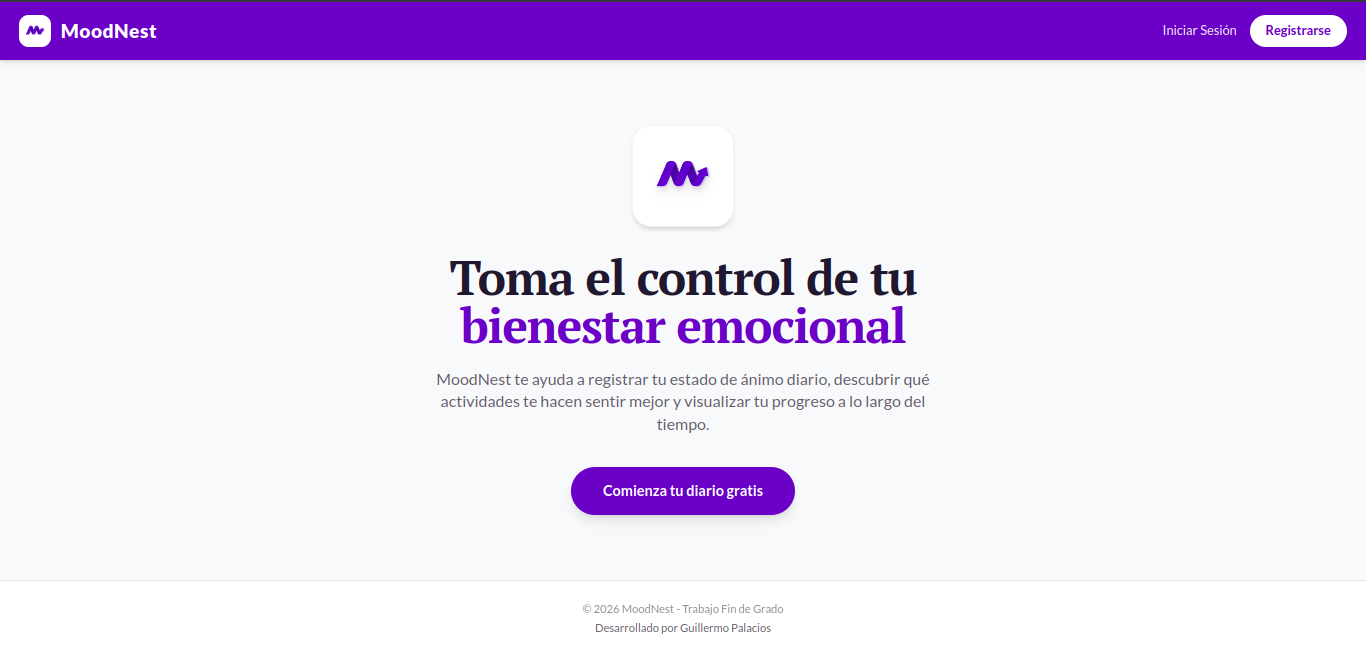
\includegraphics[width=0.85\textwidth]{Imagenes/pantalla_bienvenida.png}
    \caption{Pantalla de Bienvenida pública de MoodNest.}
    \label{fig:bienvenida}
\end{figure}

Los componentes interactivos clave distribuidos en esta vista son:
\begin{itemize}
    \item \textbf{Barra de Navegación:} Ubicada en la zona superior, expone de manera persistente dos botones de acción de alta visibilidad: ``Iniciar Sesión'' y ``Registrarse''.
    \item \textbf{Llamada a la Acción Principal:} En el centro de la pantalla se dispone el botón destacado ``Comienza tu diario gratis''. Al pulsar en este botón, el usuario será redirigido al apartado de registro para dar inicio a su aventura en MoodNest.
\end{itemize}

\subsubsection{Formularios de Acceso y Registro de Cuentas}

Al interactuar con los botones de ``Iniciar Sesión'' o ``Registrarse'', el usuario será redirigido a los apartados correspondientes para, por un lado, acceder a MoodNest con una cuenta ya existente en el sistema (Iniciar Sesión (ver Figura~\ref{fig:login})), o por otro lado, crear una nueva cuenta en el sistema (Registrarse (ver Figura~\ref{fig:registro})).

\begin{figure}[H]
    \centering
    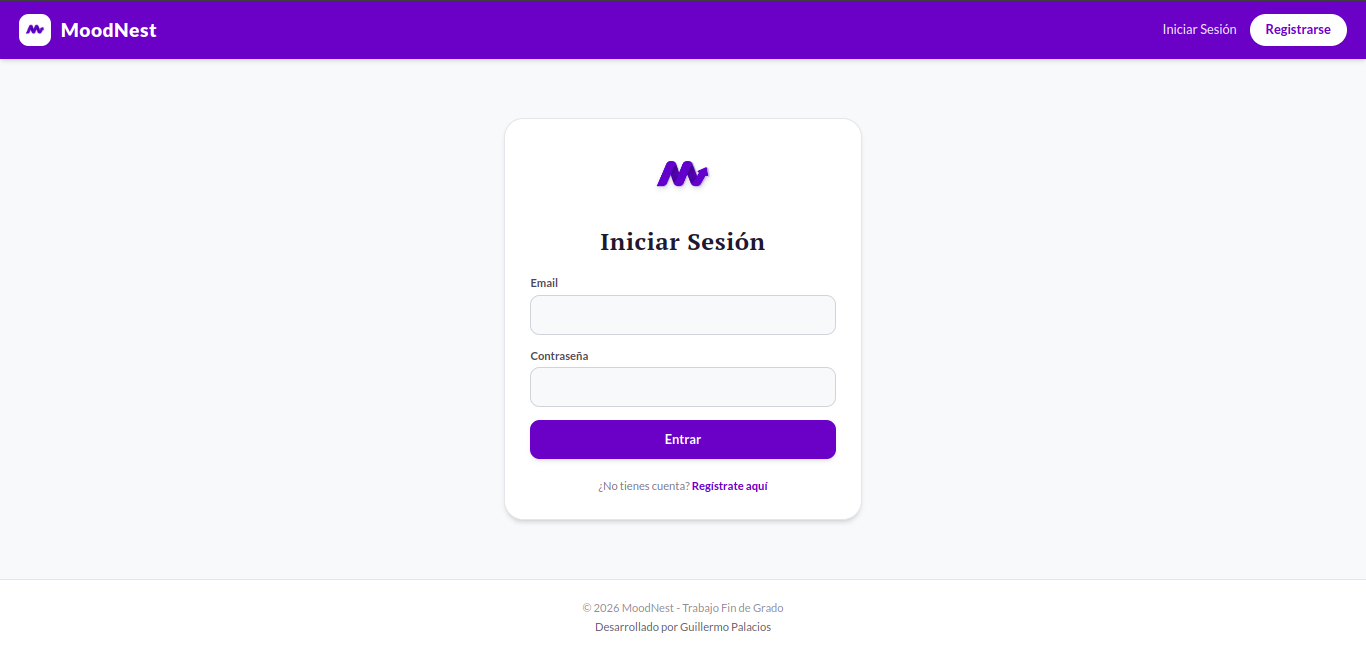
\includegraphics[width=0.85\textwidth]{Imagenes/pantalla_iniciar_sesion.png}
    \caption{Interfaz de Inicio de Sesión de MoodNest.}
    \label{fig:login}
\end{figure}

\begin{figure}[H]
    \centering
    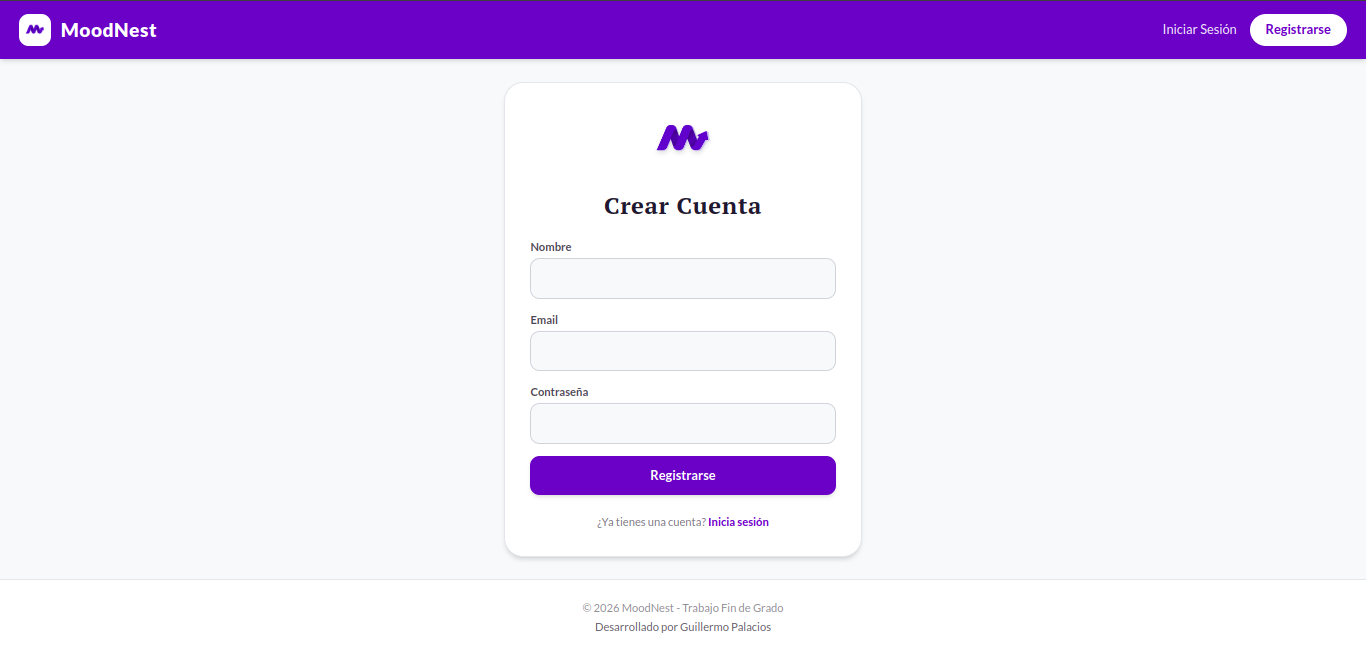
\includegraphics[width=0.85\textwidth]{Imagenes/pantalla_crear_cuenta.png}
    \caption{Interfaz de Registro de Usuario en MoodNest.}
    \label{fig:registro}
\end{figure}

Ambas vistas se estructuran mediante módulos de captura de datos validados en tiempo real:
\begin{itemize}
    \item \textbf{Campos de Entrada:} En la pantalla de inicio de sesión se solicitan obligatoriamente los campos de correo electrónico y contraseña, mientras que en la pantalla de registro se incluye también el campo de ``Nombre'', el cual representa el apodo que el usuario quiere tener dentro de MoodNest.
    \item \textbf{Enlaces de Interconexión Cruzada:} Con el fin de facilitar la navegación al usuario, la base de cada tarjeta incluye un enlace de redirección, facilitando al usuario la creación de una nueva cuenta o el acceso con una ya existente (``¿No tienes cuenta? Regístrate aquí'' y ``¿Ya tienes cuenta? Inicia sesión''), vinculando ambos estados de forma directa sin requerir volver a la página de bienvenida.
\end{itemize}

\subsection{El Panel Principal (Dashboard) Inicial}

Una vez que el usuario accede de forma exitosa en MoodNest, ya sea iniciando sesión o registrándose, será dirigido a su panel principal donde podrá comenzar su aventura en MoodNest (ver Figura~\ref{fig:dashboard_inicial}).

\begin{figure}[H]
    \centering
    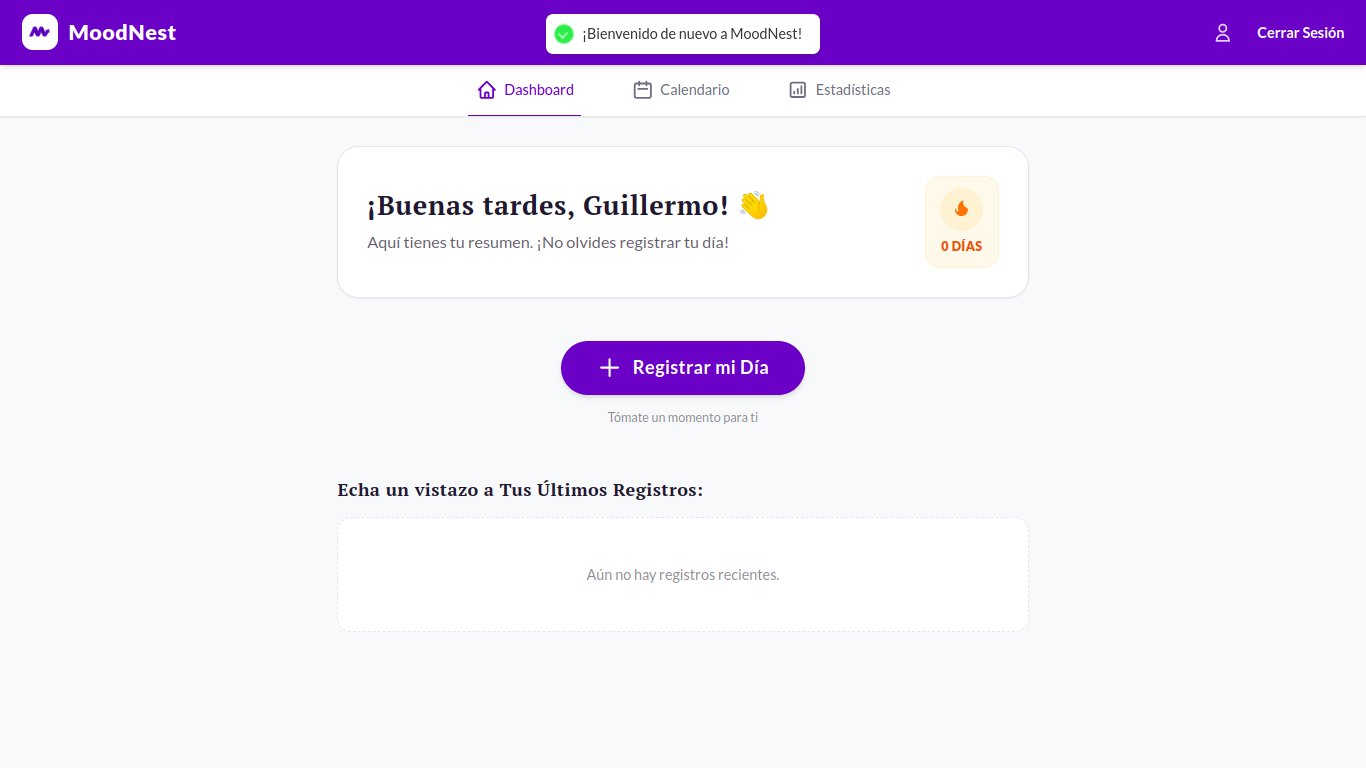
\includegraphics[width=0.85\textwidth]{Imagenes/pantalla_dashboard_inicial.png}
    \caption{Vista general del Dashboard Inicial tras el primer acceso.}
    \label{fig:dashboard_inicial}
\end{figure}

En este escenario de primera toma de contacto, destacan los siguientes elementos reactivos:
\begin{itemize}
    \item \textbf{Notificación Reactiva de Bienvenida:} Cuando el usuario interactúa con MoodNest, recibirá retroalimentación mediante notificaciones flotantes, visibles en la parte superior central de la pantalla.
    \item \textbf{Menú de Navegación Interna:} Dispuesto de forma horizontal justo debajo de la barra de navegación superior. Es el encargado de permitir al usuario moverse con facilidad entre las distintas pantallas de MoodNest (Dashboard (Actual), Calendario y Estadísticas).
    \item \textbf{Saludo Dinámico y Racha:} En la propia pantalla del Dashboard, destaca su saludo dinámico, el cual varía según la franja horaria del usuario y su nombre dentro de MoodNest y como subtítulo se muestra un mensaje que advierte al usuario de que el día está pendiente de registro. Justo en la parte derecha observaremos la racha actualizada del usuario, la cual representa el número de días registrados consecutivamente hasta la fecha actual.
    \item \textbf{Control Central de Inserción:} Se presenta el botón de gran formato ``Registrar mi Día'' como el elemento con mayor peso visual y el que permite crear los registros diarios al usuario.
\end{itemize}

\subsection{Formulario de Registro Diario y Gestión de Etiquetas}

Al presionar el botón central, la interfaz despliega una ventana modal con el formulario completo para rellenar el estado de ánimo diario del usuario. En la Figura~\ref{fig:reg_inicial} se observa el formulario inicial en blanco, mientras que en la Figura~\ref{fig:reg_rellenado} se muestra ya rellenado, con sus etiquetas asociadas y su comentario, siendo estos dos últimos opcionales.

\begin{figure}[H]
    \centering
    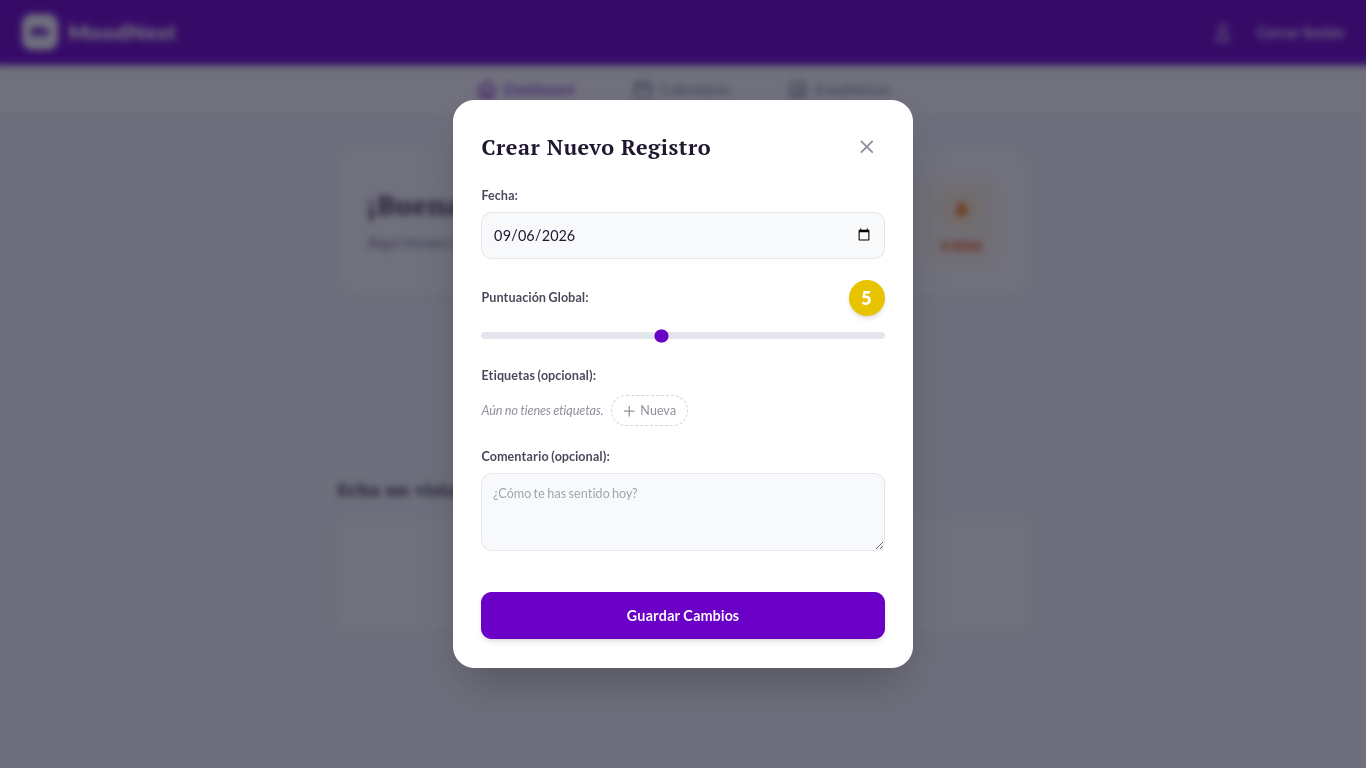
\includegraphics[width=0.85\textwidth]{Imagenes/pantalla_crear_registro_inicial.png}
    \caption{Formulario de registro diario en estado inicial.}
    \label{fig:reg_inicial}
\end{figure}

\begin{figure}[H]
    \centering
    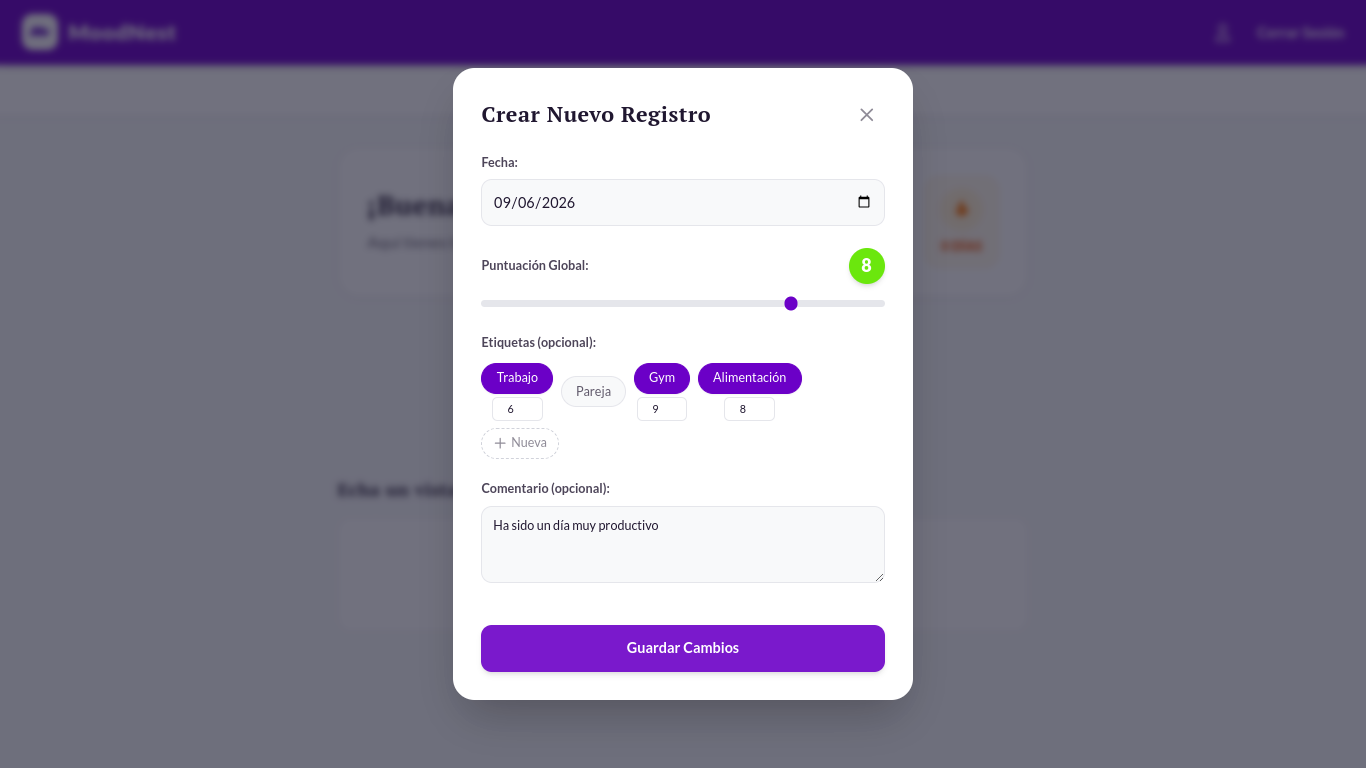
\includegraphics[width=0.85\textwidth]{Imagenes/pantalla_crear_registro_rellenado.png}
    \caption{Formulario de registro diario rellenado con sub-notas y tags evaluados.}
    \label{fig:reg_rellenado}
\end{figure}

El formulario se compone de cuatro áreas funcionales:
\begin{enumerate}
    \item \textbf{Selector Temporal de Fecha:} Preselecciona automáticamente el día actual. Permite su modificación para rellenar jornadas del pasado, bloqueando sin embargo la selección de fechas futuras.
    \item \textbf{Deslizador de Puntuación Global:} Control deslizante del 1 al 10. Al ser manipulado, el indicador numérico cambia reactivamente de color siguiendo la escala semántica emocional.
    \item \textbf{Cuadro de Selección de Etiquetas:} Las etiquetas han sido pensadas para que el usuario pueda asociar actividades, emociones, situaciones, personas, etc. Cualquier cosa que ayude a representar mejor su día. Si el usuario aún no tiene etiquetas creadas puede crearlas en el momento rápidamente y si ya tiene etiquetas creadas puede asociarlas o desactivarlas (Si ya están asociadas) de su día simplemente haciendo clic sobre ellas. Además al asociar una etiqueta, será posible la opción de incluirle una puntuación a dicha etiqueta de forma completamente opcional.
    \item \textbf{Comentario Textual:} Área libre completamente opcional para aquellas anotaciones extra o de diario que el usuario quiera incluir sobre su día.
\end{enumerate}

\subsection{Panel Principal (Dashboard) Post-Registro}

Una vez que el usuario presiona ``Guardar Registro'', la información es procesada y guardada en el historial del usuario. De inmediato, la aplicación actualiza el panel principal para reflejar el cambio de estado (ver Figura~\ref{fig:dashboard_post}).

\begin{figure}[H]
    \centering
    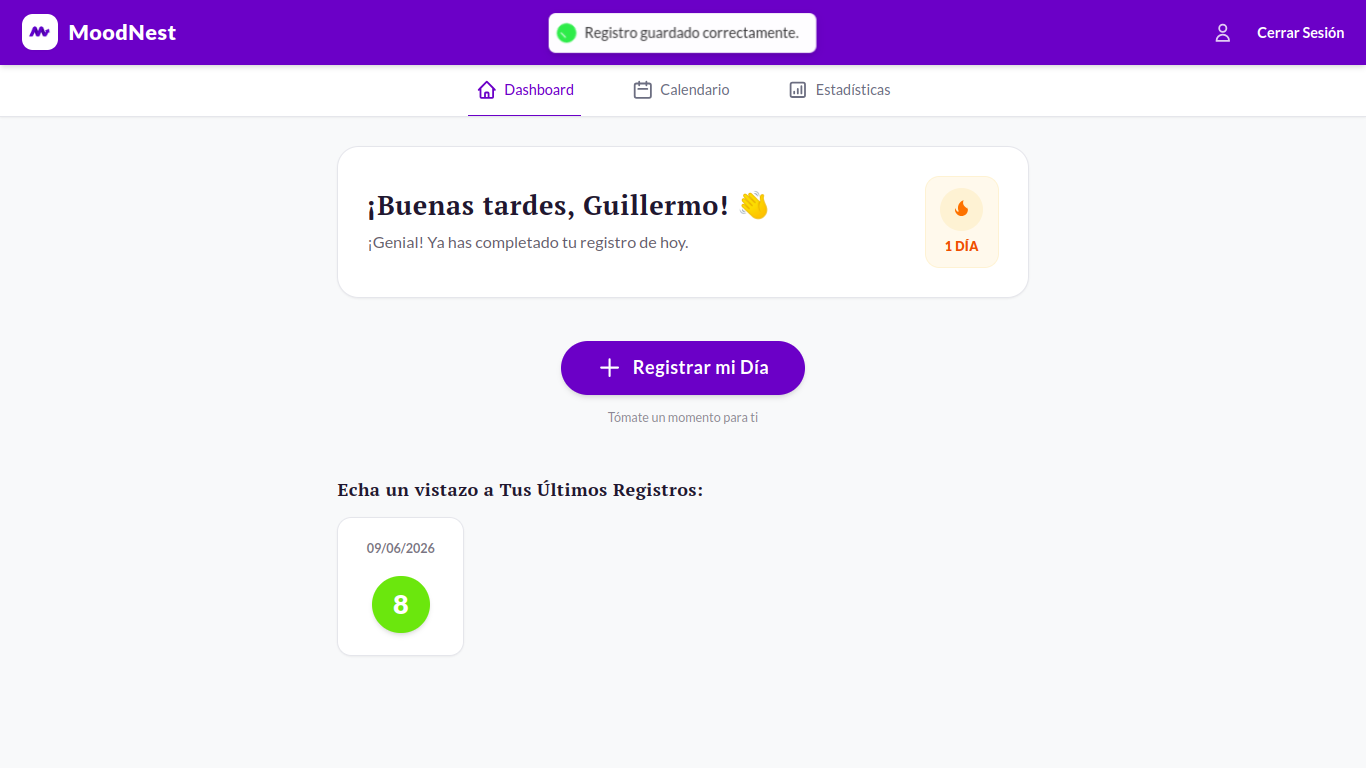
\includegraphics[width=0.85\textwidth]{Imagenes/pantalla_dashboard_postregistro.png}
    \caption{Estado del Dashboard tras consolidar el registro diario.}
    \label{fig:dashboard_post}
\end{figure}

Las actualizaciones automáticas del sistema visibles en este panel corresponden a:
\begin{itemize}
    \item \textbf{Actualización de Métricas Dinámicas:} El saludo felicita proactivamente al usuario por haber completado la jornada y el contador de racha incrementa su valor de forma inmediata a \texttt{1 día}.
    \item \textbf{Bloque de Últimos Registros:} En la parte final de la pantalla aparecerá una nueva tarjeta interactiva correspondiente al registro recién creado. Esta tarjeta visualiza la fecha formateada y la nota global encerrada en el color semántico asociado.
    \item \textbf{Visualización de Detalles:} Si el usuario interactúa haciendo clic sobre cualquiera de las tarjetas de las últimas entradas registradas, será redirigido hacia la pantalla de Historial y cargando los detalles del registro.
\end{itemize}

\subsection{Historial y Navegación Cronológica mensual}

La pantalla de Historial se plantea como un visor mensual interactivo estructurado en una disposición de doble columna responsiva. La Figura~\ref{fig:hist_con} muestra la inspección de un día con datos, y la Figura~\ref{fig:hist_sin} el estado ante un día vacío.

\begin{figure}[H]
    \centering
    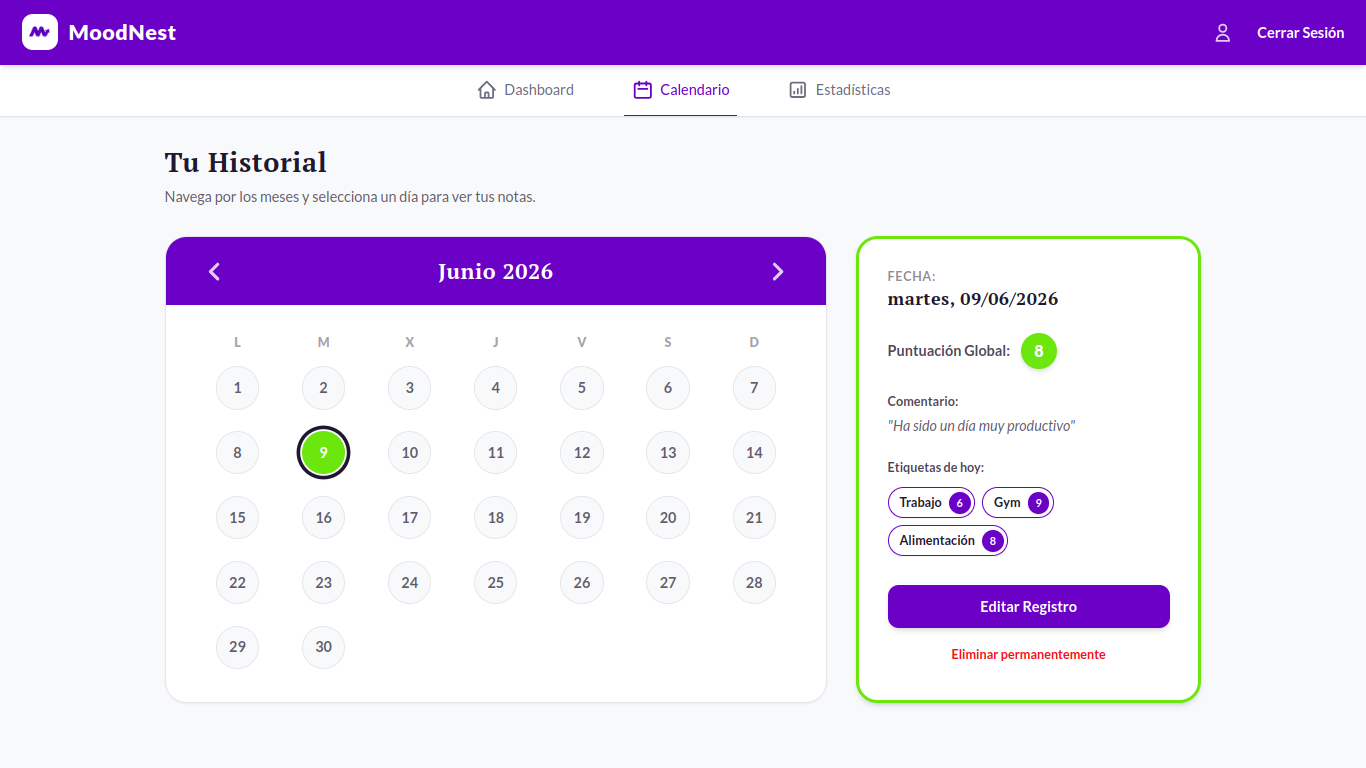
\includegraphics[width=0.85\textwidth]{Imagenes/pantalla_historial_postregistro.png}
    \caption{Vista de Historial: Inspección de un día con registro consolidado.}
    \label{fig:hist_con}
\end{figure}

\begin{figure}[H]
    \centering
    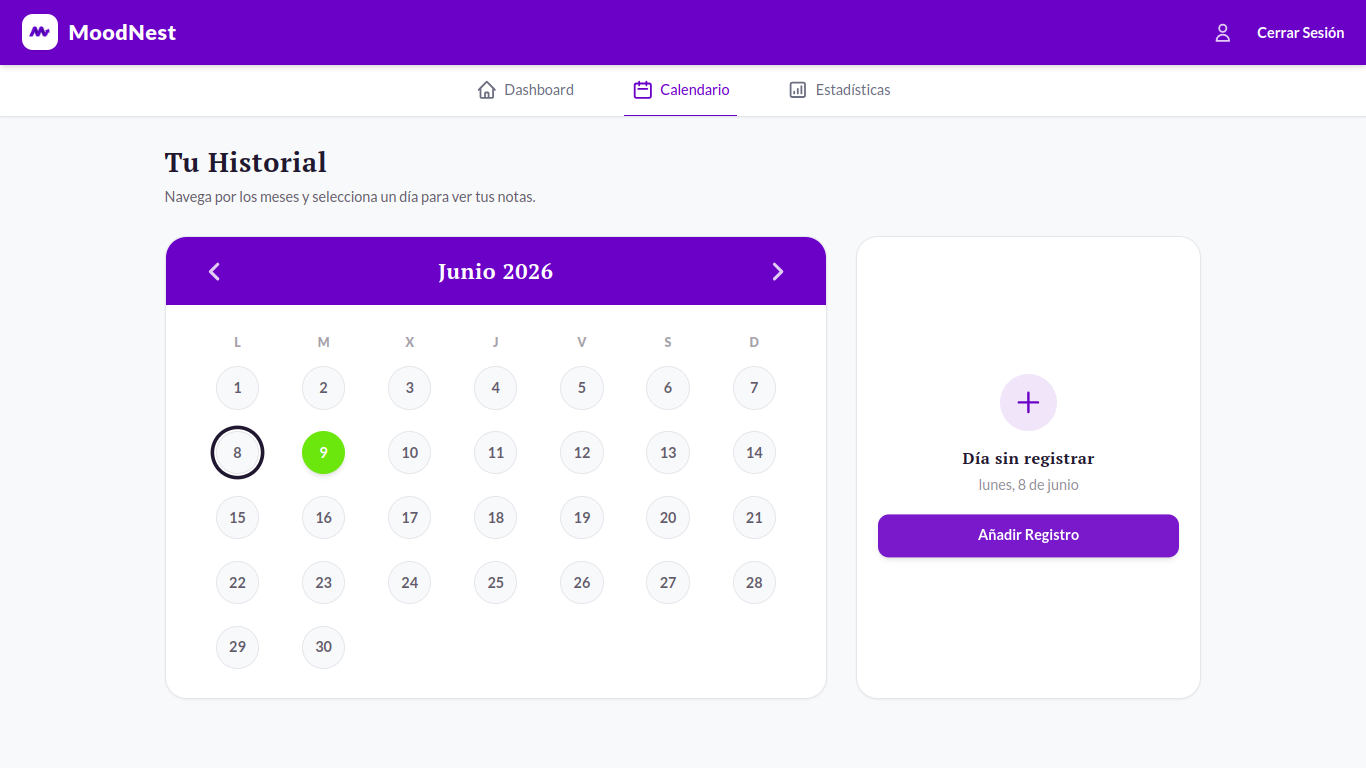
\includegraphics[width=0.85\textwidth]{Imagenes/pantalla_historial_diaSinRegistro.png}
    \caption{Vista de Historial: Panel derecho ante un día sin registro.}
    \label{fig:hist_sin}
\end{figure}

El comportamiento de este componente se rige por las siguientes interacciones:
\begin{itemize}
    \item \textbf{Navegación del Calendario (Columna Izquierda):} El usuario puede navegar entre meses utilizando las flechas del encabezado, para ver su historial completo de registros de un mes cualquiera. 
    \item \textbf{Panel Contextual de Inspección (Columna Derecha):} Al hacer clic sobre una celda del calendario, la columna derecha reacciona según la existencia de datos:
    \begin{itemize}
        \item \textbf{Día con registro:} Detalla la puntuación global, el comentario y el listado de etiquetas evaluadas. Habilita los botones para ``Editar'' y ``Eliminar'' dicho registro.
        \item \textbf{Día sin registro:} Muestra un estado vacío explicativo con un botón de inserción rápida configurado con la fecha de la celda seleccionada, para que el usuario añada un registro para ese día si así lo desea.
    \end{itemize}
\end{itemize}

\subsection{Panel de Configuración y Perfil de Usuario}

La vista de Perfil cede el gobierno absoluto de la aplicación al usuario autenticado, agrupando sus capacidades operativas en diferentes bloques de gestión (ver Figuras~\ref{fig:perf_ini} a~\ref{fig:perf_logout}).

\begin{figure}[H]
    \centering
    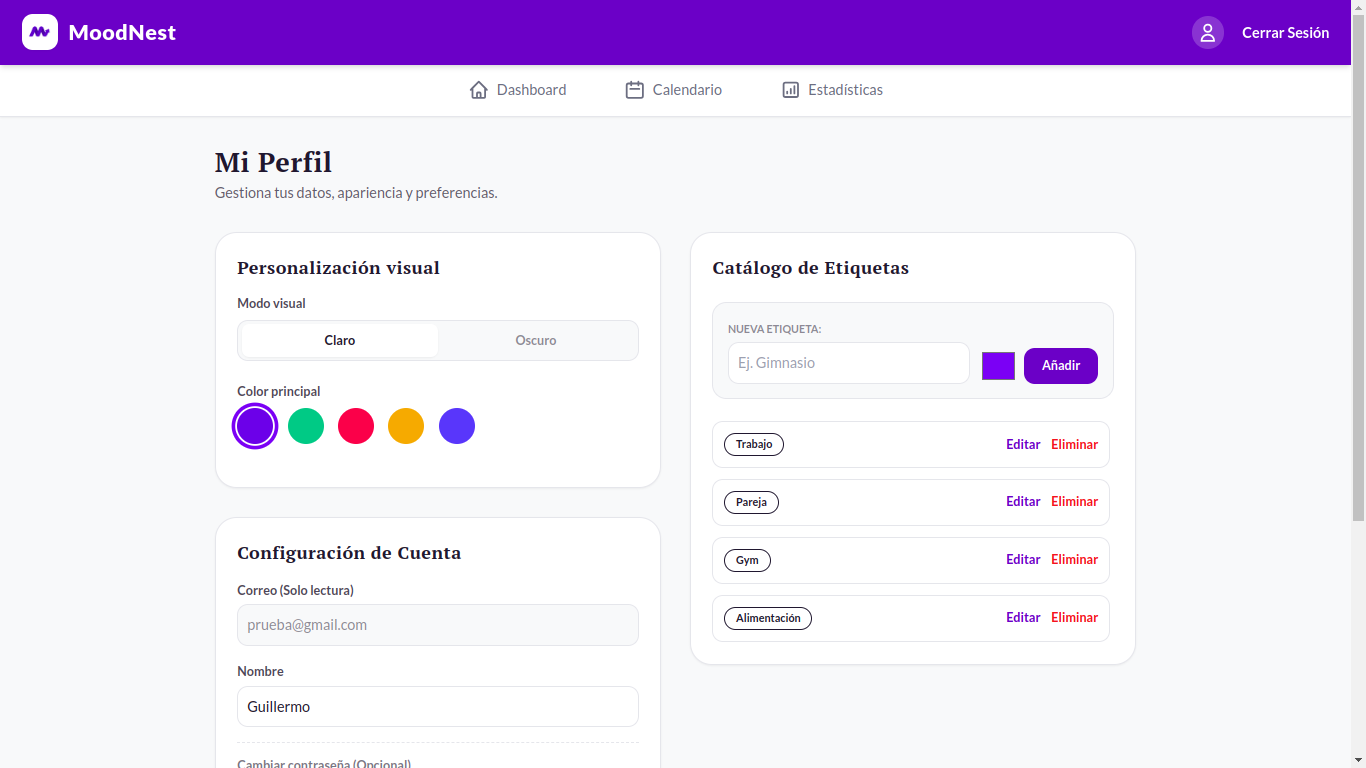
\includegraphics[width=0.85\textwidth]{Imagenes/pantalla_perfil_inicial.png}
    \caption{Vista general del panel de Perfil del usuario.}
    \label{fig:perf_ini}
\end{figure}

\begin{figure}[H]
    \centering
    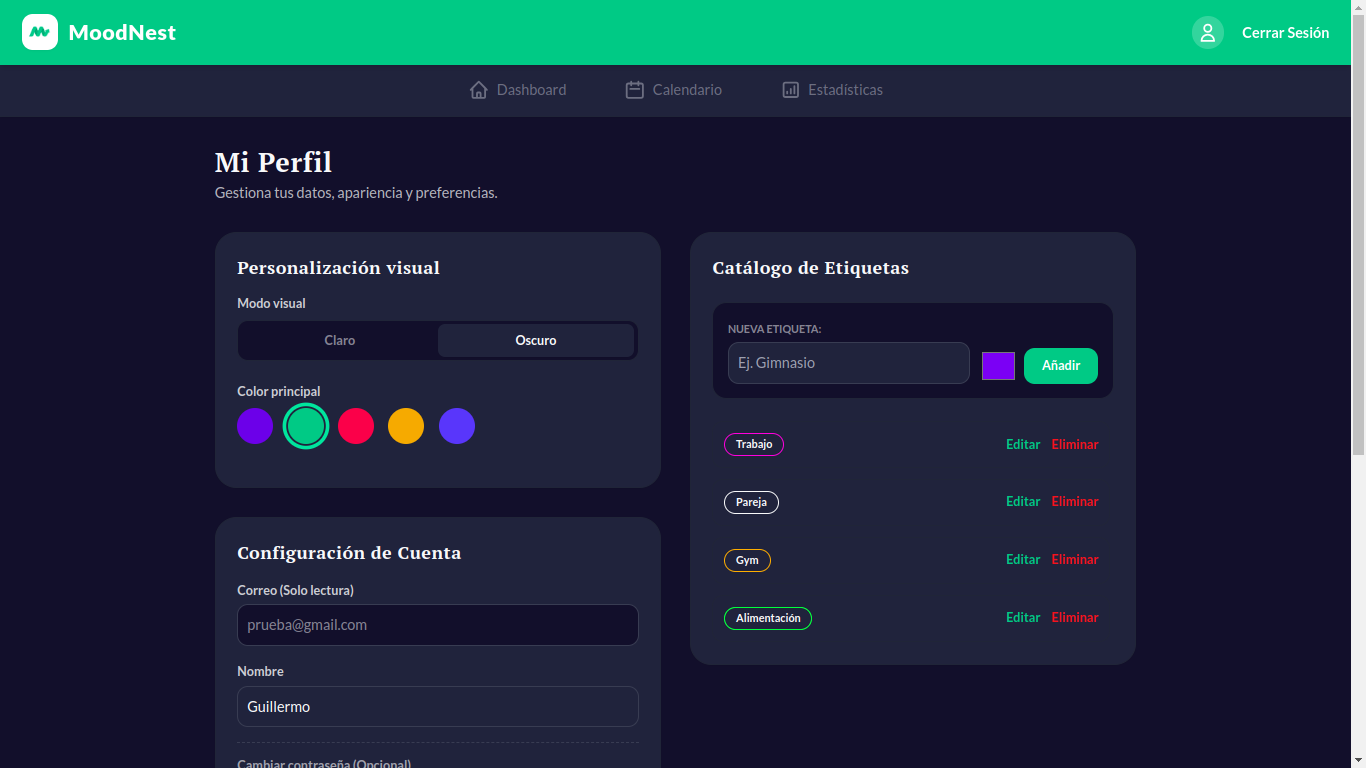
\includegraphics[width=0.85\textwidth]{Imagenes/pantalla_perfil_personalizarInterfaz.png}
    \caption{Widget de personalización estética de la interfaz (Tema y Color).}
    \label{fig:perf_inter}
\end{figure}

\begin{figure}[H]
    \centering
    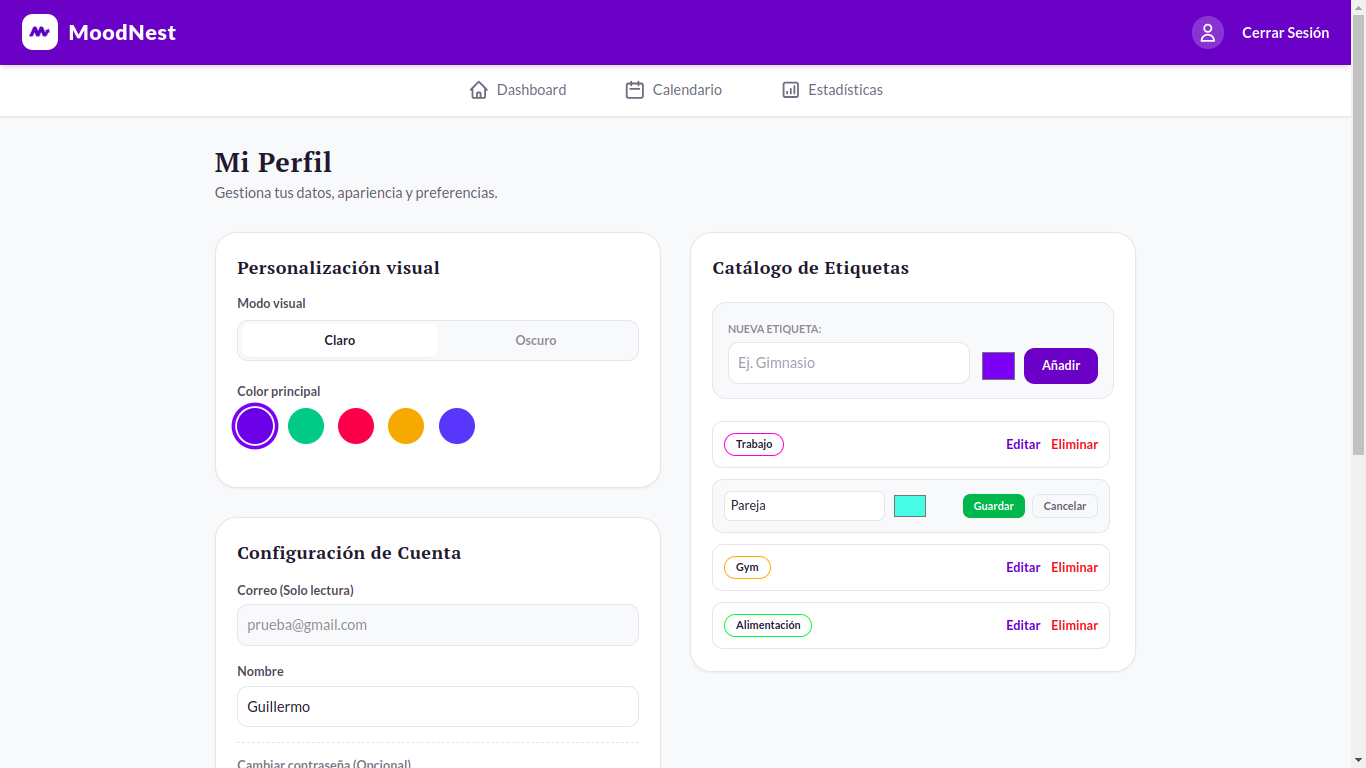
\includegraphics[width=0.85\textwidth]{Imagenes/pantalla_perfil_editarEtiqueta.png}
    \caption{Módulo de gestión y edición del catálogo de etiquetas.}
    \label{fig:perf_etiq}
\end{figure}

\begin{figure}[H]
    \centering
    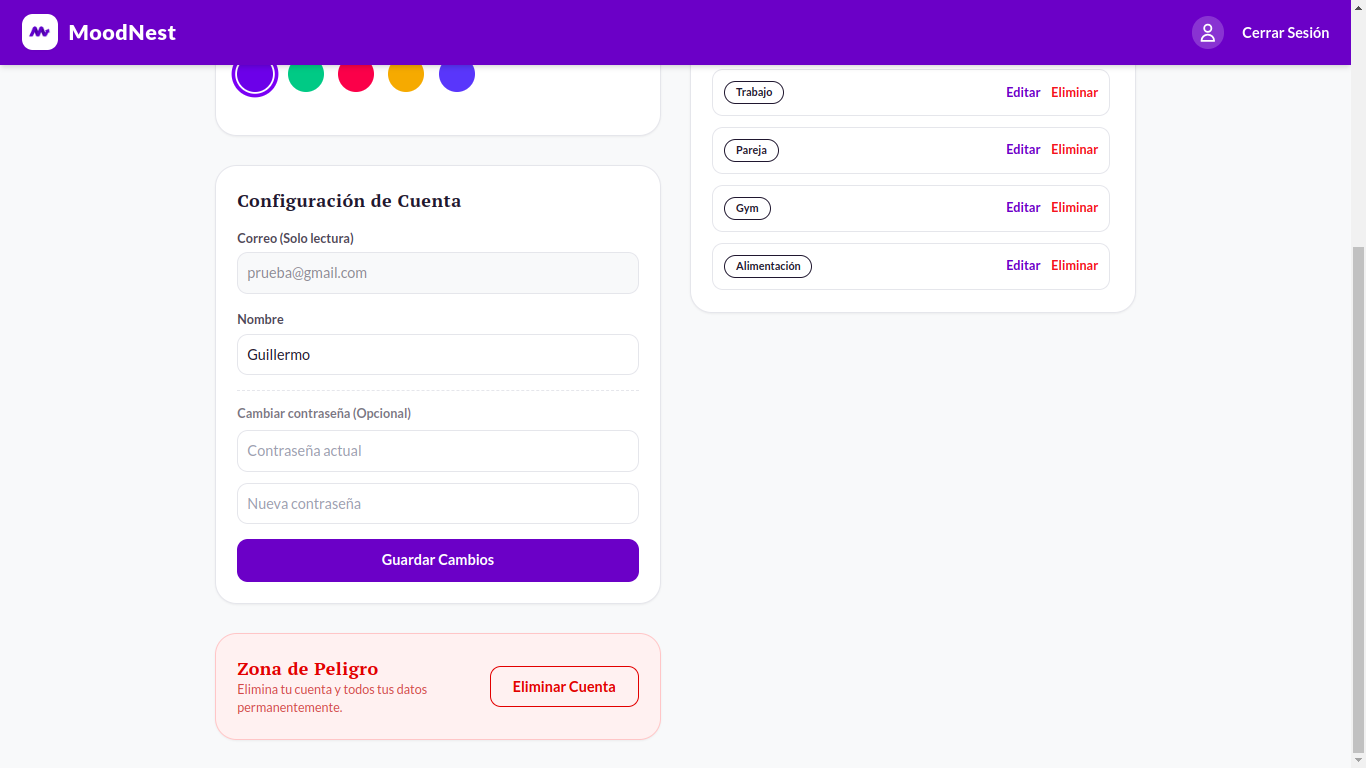
\includegraphics[width=0.85\textwidth]{Imagenes/pantalla_perfil_configuracionCuenta.png}
    \caption{Formularios de seguridad y actualización de credenciales.}
    \label{fig:perf_cuenta}
\end{figure}

Las funcionalidades desplegadas de forma atómica en este panel comprenden:
\begin{enumerate}
    \item \textbf{Personalización de la Interfaz (Figura~\ref{fig:perf_inter}):} Expone un conmutador semántico para alternar entre el Modo Claro y el Modo Oscuro, y una paleta de colores para reconfigurar el color principal de la interfaz.
    \item \textbf{Gestión de Catálogo de Etiquetas (Figura~\ref{fig:perf_etiq}):} Muestra el listado de las etiquetas personalizadas activas del usuario además de permitir la creación, edición y eliminación de las mismas mediante los botones de ``Añadir'', ``Editar'' y ``Eliminar''.
    \item \textbf{Configuración de la Cuenta (Figura~\ref{fig:perf_cuenta}):} Permite al usuario actualizar de manera independiente el nombre o la contraseña si así lo desea.
    \item \textbf{Eliminación de la Cuenta:} Acotado visualmente dentro de una ``Zona de Peligro'' (ver Figura~\ref{fig:perf_elim}). Al hacer clic en esta, el usuario deberá introducir su contraseña actual y así confirmar que realmente desea eliminar por completo su cuenta de MoodNest y todo su historial.
\end{enumerate}

\begin{figure}[H]
    \centering
    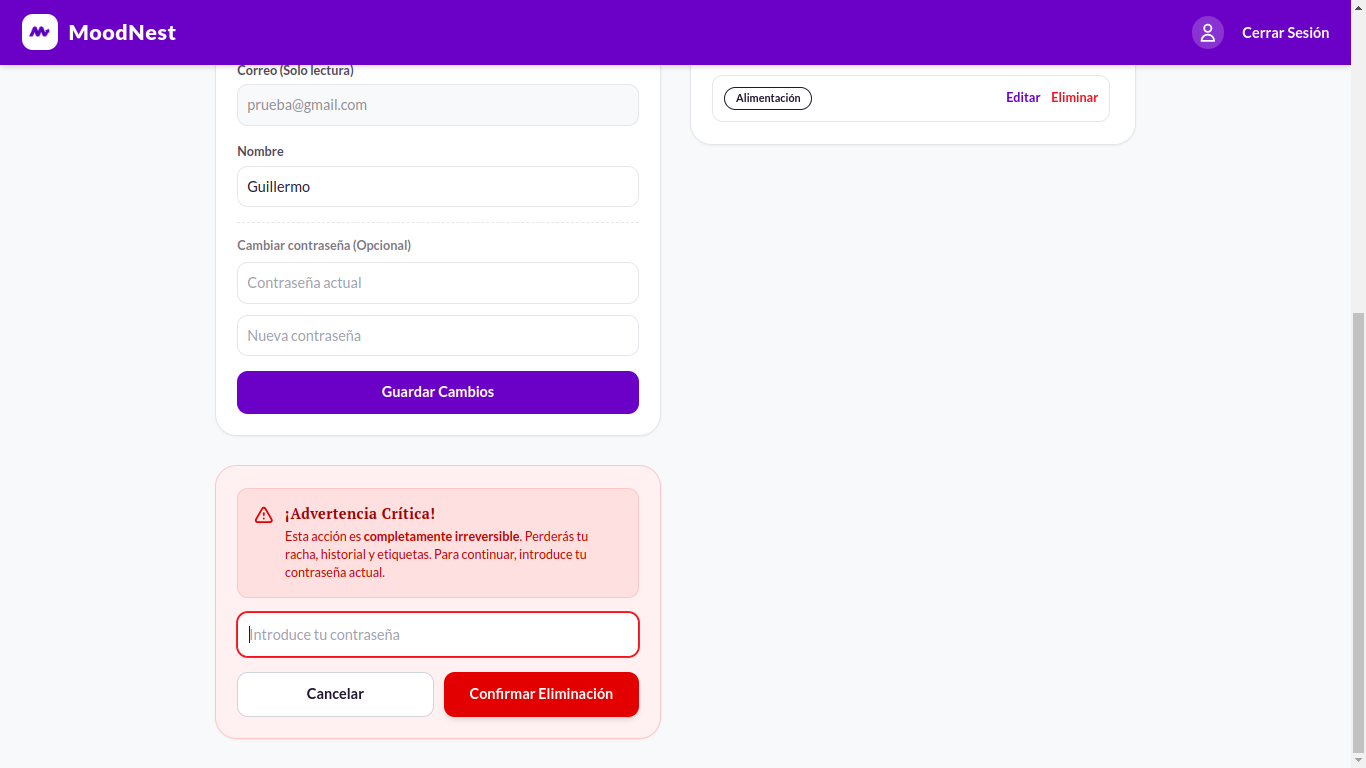
\includegraphics[width=0.85\textwidth]{Imagenes/pantalla_perfil_eliminarCuenta.png}
    \caption{Widget crítico de confirmación para la eliminación de la cuenta.}
    \label{fig:perf_elim}
\end{figure}

\subsection{Módulo Analítico y Estadísticas Avanzadas}

El panel de estadísticas representa el núcleo de MoodNest, traduciendo los registros diarios del usuario en conclusiones de valor sobre su bienestar.

\subsubsection{Comportamiento en Ausencia de Datos (Estado Vacío)}

Inicialmente, para usuario recién registrado en MoodNest que aún no cuenta con registros en su historial, la interfaz del sistema mostrará cuadros vacíos avisando al usuario de la falta de registros en su historial (ver Figuras~\ref{fig:est_vac1} y~\ref{fig:est_vac2}).

\begin{figure}[H]
    \centering
    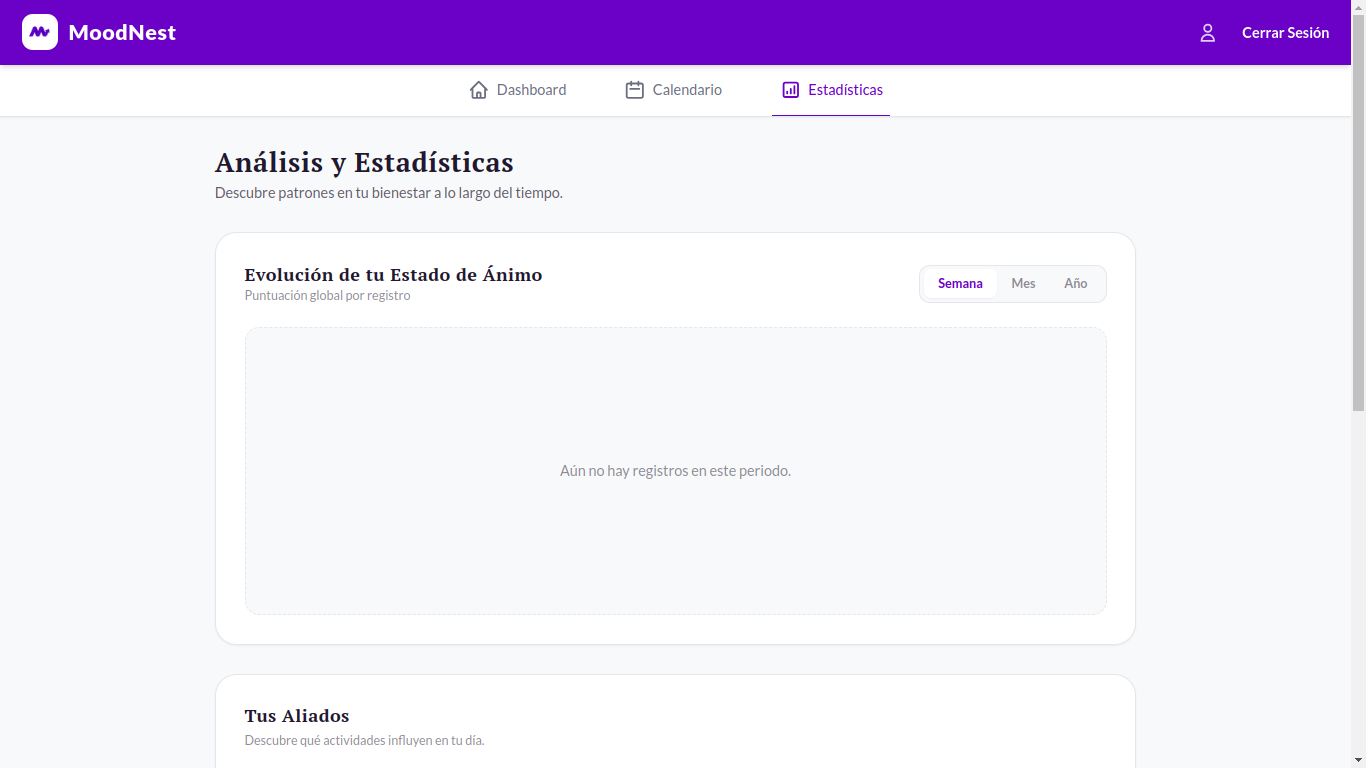
\includegraphics[width=0.85\textwidth]{Imagenes/pantalla_estadisticas_inicial_1.png}
    \caption{Estado inicial de estadísticas: Bloque cronológico superior vacío.}
    \label{fig:est_vac1}
\end{figure}

\begin{figure}[H]
    \centering
    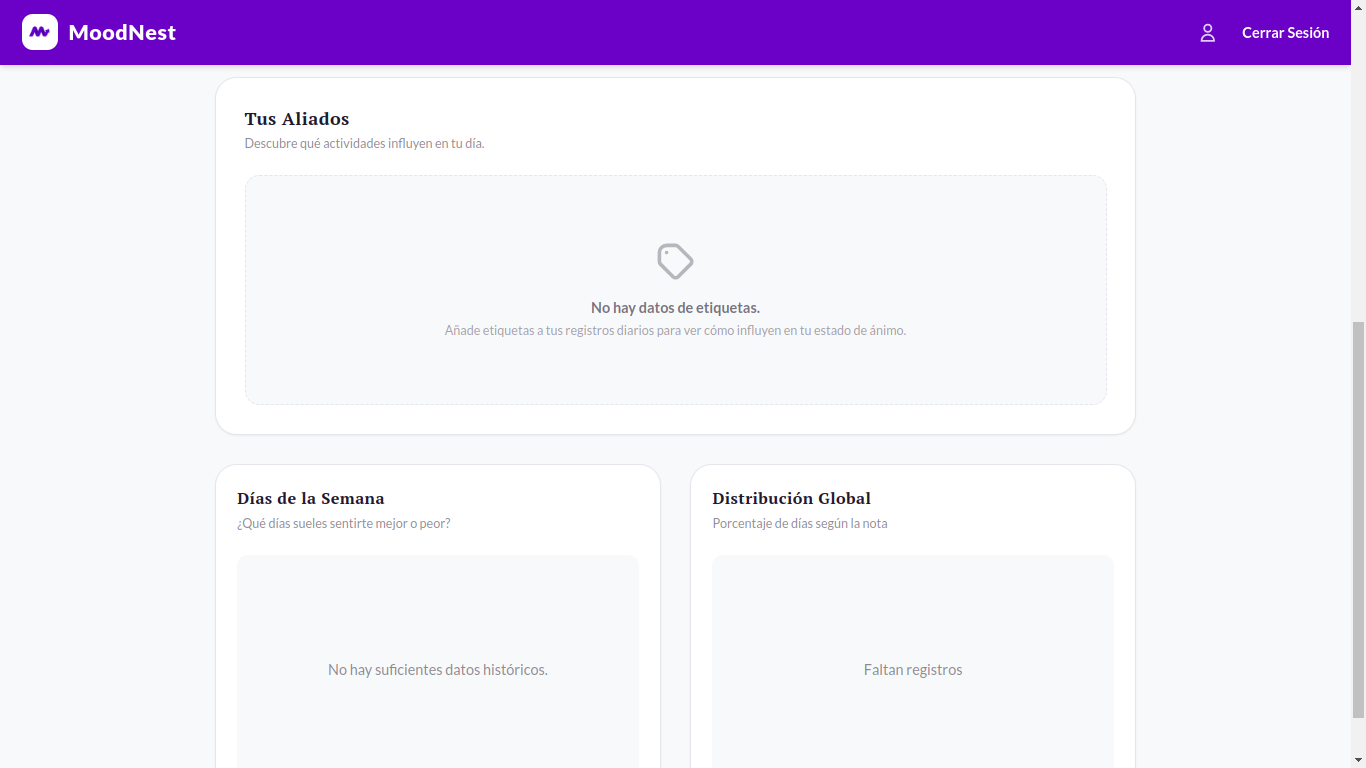
\includegraphics[width=0.85\textwidth]{Imagenes/pantalla_estadisticas_inicial_2.png}
    \caption{Estado inicial de estadísticas: Paneles analíticos de tags vacíos.}
    \label{fig:est_vac2}
\end{figure}

\subsubsection{Visualización Avanzada tras Uso Continuo}

Tras recopilar registros durante varios días o semanas, el módulo analítico se hidrata por completo y procesa todos y cada uno de los registros creados por el usuario, distribuyendo la información en tres secciones (ver Figuras~\ref{fig:est_sem} a~\ref{fig:est_dist}).

\begin{figure}[H]
    \centering
    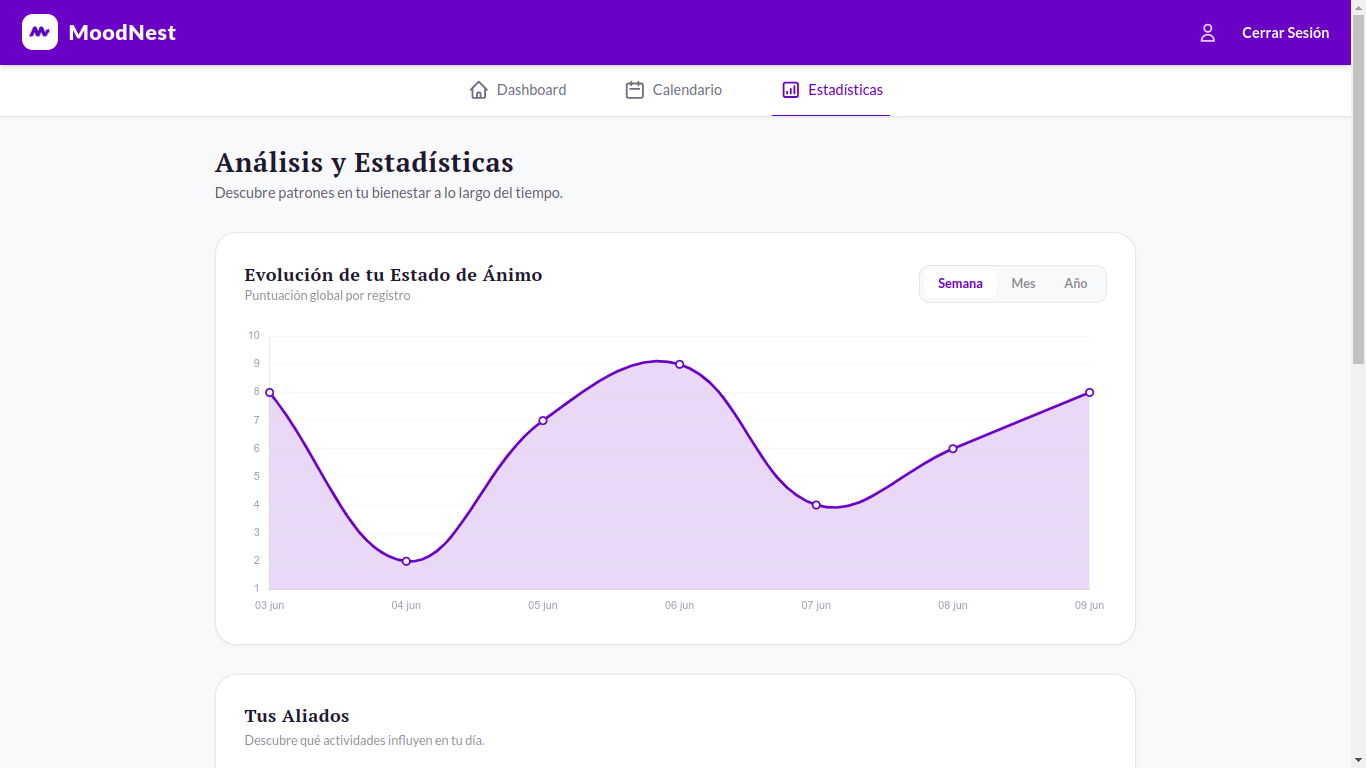
\includegraphics[width=0.85\textwidth]{Imagenes/pantalla_estadisticas_semanal.png}
    \caption{Gráfico de evolución temporal con filtro semanal activado.}
    \label{fig:est_sem}
\end{figure}

\begin{figure}[H]
    \centering
    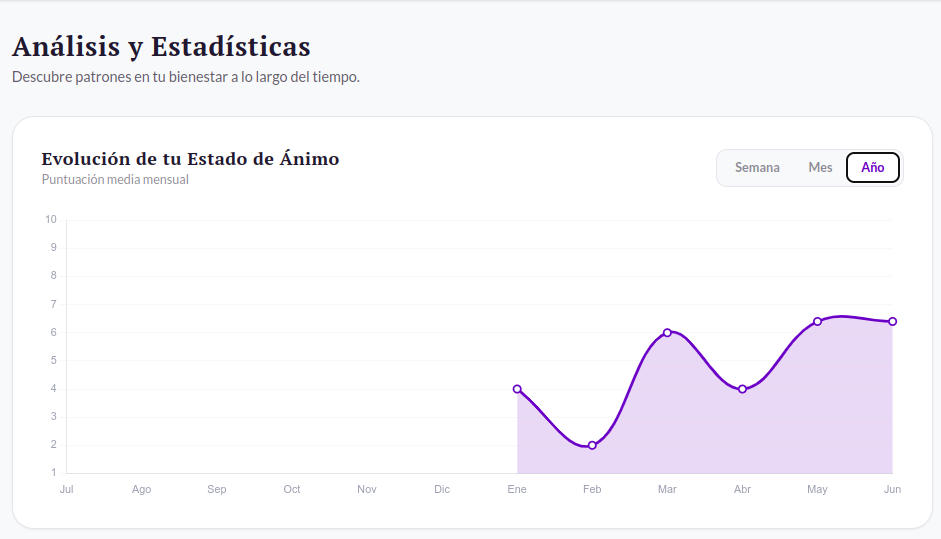
\includegraphics[width=0.85\textwidth]{Imagenes/pantalla_estadisticas_anual.png}
    \caption{Gráfico de evolución temporal con filtro anual activado.}
    \label{fig:est_anual}
\end{figure}

\begin{figure}[H]
    \centering
    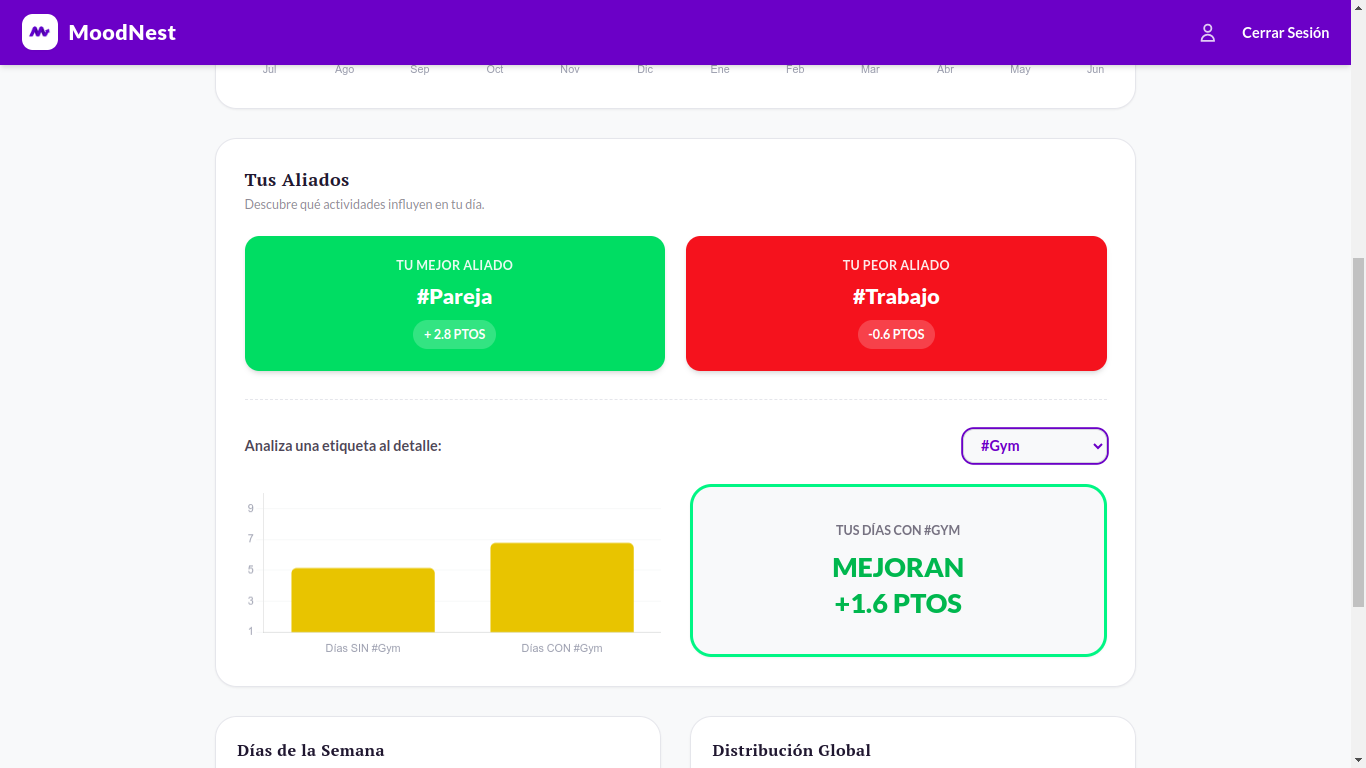
\includegraphics[width=0.85\textwidth]{Imagenes/pantalla_estadisticas_aliados.png}
    \caption{Métricas de correlación extrema de etiquetas (Aliados).}
    \label{fig:est_aliados}
\end{figure}

\begin{figure}[H]
    \centering
    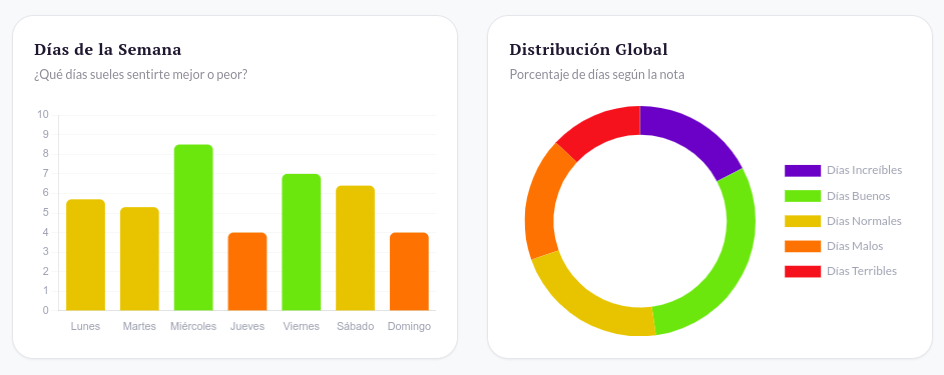
\includegraphics[width=0.85\textwidth]{Imagenes/pantalla_estadisticas_diasSemanaYPromedio.png}
    \caption{Distribuciones avanzadas: Barras por día y Anillo de promedio cualitativo.}
    \label{fig:est_dist}
\end{figure}

Los cuatro bloques funcionales operan bajo las siguientes premisas técnicas:
\begin{enumerate}
    \item \textbf{Evolución Temporal del Estado de Ánimo (Figuras~\ref{fig:est_sem} y~\ref{fig:est_anual}):} En esta sección se refleja la evolución temporal del estado de ánimo del usuario, pudiendo ver las fluctuaciones de su estado de ánimo a lo largo de la última semana, último mes y último año.
    \item \textbf{Módulo Central ``Tus Aliados'' (Figura~\ref{fig:est_aliados}):} En la parte superior de esta sección se muestran las dos etiquetas con mayor impacto en el estado de ánimo diario del usuario. En la parte izquierda se muestra la etiqueta con mayor impacto positivo y en la parte derecha se muestra la etiqueta con mayor impacto negativo, ambas acompañadas del impacto exacto en la puntuación diaria del usuario. Por otro lado, en la parte inferior el usuario puede valorar el impacto de una etiqueta concreta cualquiera, siempre y cuando exista al menos un registro con dicha etiqueta asociada y otro registro sin ella. La interfaz muestra un gráfico de barras comparativo entre la media de la puntuación global de los días sin la etiqueta y de los días con la etiqueta y justamente en la parte derecha, un mensaje dinámico sobre el resultado obtenido.
    \item \textbf{Distribuciones y Tendencias (Figura~\ref{fig:est_dist}):} En la parte final de las estadísticas, se encuentran dos gráficos. El de la izquierda permitirá al usuario conocer la tendencia de su estado de ánimo según el día de la semana, mientras que el de la derecha muestra la distribución porcentual del total de días registrados en el sistema agrupados por: días increíbles (puntuaciones de 9 y 10), buenos (puntuaciones de 7 y 8), normales (puntuaciones de 5 y 6), malos (puntuaciones de 3 y 4) y terribles (puntuaciones de 1 y 2).
\end{enumerate}

\subsection{Finalización de Sesión Segura}

El usuario autenticado dispone en todo momento del control para efectuar un cierre de sesión y asegurar así la privacidad de su información. Esta funcionalidad, se encuentra accesible en la zona lateral derecha de la barra superior de navegación, donde aparece exactamente el texto de ``Cerrar Sesión''.

Al interactuar con dicho elemento, la interfaz despliega una ventana modal de confirmación previa a la salida (ver Figura~\ref{fig:perf_logout}). Si el usuario ratifica la acción, el sistema mantendrá la privacidad del usuario y será redirigido nuevamente a la pantalla de bienvenida (Figura~\ref{fig:bienvenida}).


\begin{figure}[H]
    \centering
    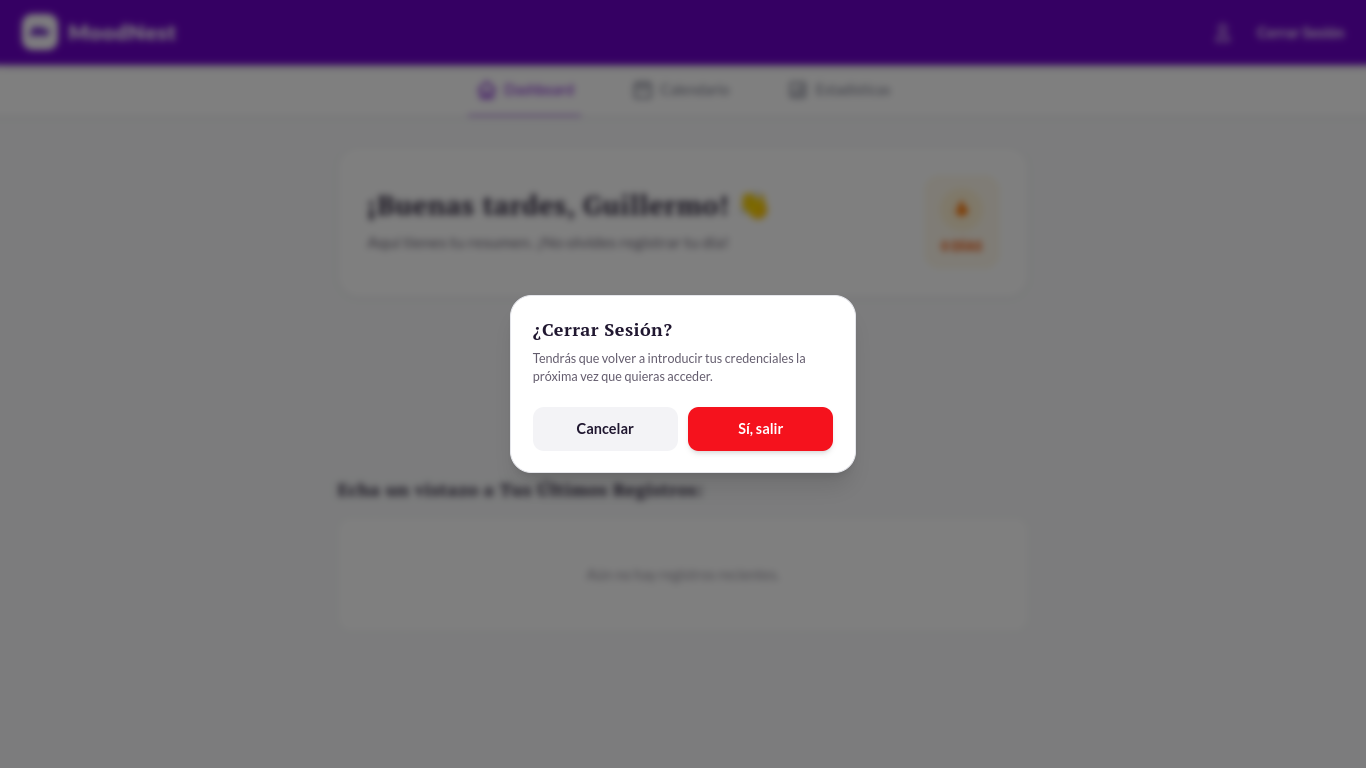
\includegraphics[width=0.85\textwidth]{Imagenes/pantalla_cerrar_sesion.png}
    \caption{Ventana modal de confirmación de Cierre de Sesión.}
    \label{fig:perf_logout}
\end{figure}


\end{document}
